%% BioMed_Central_Tex_Template_v1.06
%%                                      %
%  bmc_article.tex            ver: 1.06 %
%                                       %

%%IMPORTANT: do not delete the first line of this template
%%It must be present to enable the BMC Submission system to
%%recognise this template!!

%%%%%%%%%%%%%%%%%%%%%%%%%%%%%%%%%%%%%%%%%
%%                                     %%
%%  LaTeX template for BioMed Central  %%
%%     journal article submissions     %%
%%                                     %%
%%          <8 June 2012>              %%
%%                                     %%
%%                                     %%
%%%%%%%%%%%%%%%%%%%%%%%%%%%%%%%%%%%%%%%%%


%%%%%%%%%%%%%%%%%%%%%%%%%%%%%%%%%%%%%%%%%%%%%%%%%%%%%%%%%%%%%%%%%%%%%
%%                                                                 %%
%% For instructions on how to fill out this Tex template           %%
%% document please refer to Readme.html and the instructions for   %%
%% authors page on the biomed central website                      %%
%% http://www.biomedcentral.com/info/authors/                      %%
%%                                                                 %%
%% Please do not use \input{...} to include other tex files.       %%
%% Submit your LaTeX manuscript as one .tex document.              %%
%%                                                                 %%
%% All additional figures and files should be attached             %%
%% separately and not embedded in the \TeX\ document itself.       %%
%%                                                                 %%
%% BioMed Central currently use the MikTex distribution of         %%
%% TeX for Windows) of TeX and LaTeX.  This is available from      %%
%% http://www.miktex.org                                           %%
%%                                                                 %%
%%%%%%%%%%%%%%%%%%%%%%%%%%%%%%%%%%%%%%%%%%%%%%%%%%%%%%%%%%%%%%%%%%%%%

%%% additional documentclass options:
%  [doublespacing]
%  [linenumbers]   - put the line numbers on margins

%%% loading packages, author definitions

%\documentclass[twocolumn]{bmcart}% uncomment this for twocolumn layout and comment line below
\documentclass{bmcart}

%%% Load packages
%\usepackage{amsthm,amsmath}
%\RequirePackage{natbib}
%\RequirePackage[authoryear]{natbib}% uncomment this for author-year bibliography
%\RequirePackage{hyperref}
\usepackage[utf8]{inputenc} %unicode support
%\usepackage[applemac]{inputenc} %applemac support if unicode package fails
%\usepackage[latin1]{inputenc} %UNIX support if unicode package fails

% Packages
\usepackage{latexsym}
\usepackage{epic,eepic}
\usepackage{times}
\usepackage{amsmath}
\usepackage{amsfonts}
\usepackage{multirow}
\usepackage{graphicx}
\usepackage{algorithm}
\usepackage{algpseudocode}
\usepackage{xcolor}
\usepackage{ulem}
\usepackage{amssymb}

% Tunning
%------------------
\usepackage[12pt]{moresize}
\let\labelindent\relax
\usepackage{enumitem}
\algtext*{EndIf}% Remove "end if" text
\algtext*{EndFor}% Remove "end if" text
%\setlength{\belowcaptionskip}{10.0pt}
%\setlength{\abovecaptionskip}{10.0pt}
%\setlength{\textfloatsep}{10.0pt}
%\setlength{\floatsep}{10.0pt}
% TUNNING
%\setstretch{0.94}
%\fontsize{3.85mm}{3.85mm}\selectfont


\newcommand{\pf}[1]{\langle#1\rangle}
\newcommand{\noproof}{\hfill $qed$}
\newcommand{\ignore}[1]{}

\definecolor{gray50}{gray}{0.15}
\definecolor{verylightgray}{gray}{0.90}


\newtheorem{definition}{Definition} % [section]
\newtheorem{example}{Example} % [section]
\newtheorem{Lemma}{Lemma} % [section]

\newcommand{\pivot}[1]{\mathbin{\, {#1} \,}}
\newcommand{\Pivot}[1]{\mathbin{\; {#1} \;}}
\let\from=\leftarrow

% Pretty ref
\usepackage{prettyref}
\newrefformat{def}{Definition~\ref{#1}}
\newrefformat{fig}{Figure~\ref{#1}}
\newrefformat{tab}{Table~\ref{#1}}
%%\newrefformat{pro}{Property~\ref{#1}}
%%\newrefformat{pps}{Proposition~\ref{#1}}
%\newrefformat{lem}{Lemma~\ref{#1}}
%\newrefformat{th}{Theorem~\ref{#1}}
%\newrefformat{sec}{Section~\ref{#1}}
%%\newrefformat{subsec}{Subsect.~\ref{#1}}
%%\newrefformat{suppl}{Appendix~\ref{#1}}
\newrefformat{ex}{Example~\ref{#1}}
%%\newrefformat{eq}{Eq.~\eqref{#1}}
\newrefformat{alg}{Algorithm~\ref{#1}}
\def\pref{\prettyref}

%Algorithme
\usepackage{algorithm}
\usepackage{algpseudocode}


%Package CAV
\usepackage[english]{babel}
\usepackage{stmaryrd} % Maths (crochets doubles)
\usepackage{url}     % Mise en forme + liens pour URLs
%\usepackage{array}   % Tableaux évolués
\usepackage{setspace}

% Commande perso
\newcommand{\ie}{i.e.,\ }
\newcommand{\eg}{e.g.,\ }
\newcommand{\resp}{resp.\ }
\newcommand{\nbld}{\nobreakdash--}
\newcommand{\refl}[1]{line~\ref{#1}}
\newcommand{\refll}[2]{lines~\ref{#1}\nobreakdash--\ref{#2}}
\newcommand{\Refl}[1]{Line~\ref{#1}}
\newcommand{\Refll}[2]{Lines~\ref{#1}\nobreakdash--\ref{#2}}



% Citation
\usepackage{cite}

%marge
\newenvironment{changemargin}[2]{\begin{list}{}{%
\setlength{\topsep}{0pt}%
\setlength{\leftmargin}{0pt}%
\setlength{\rightmargin}{0pt}%
\setlength{\listparindent}{\parindent}%
\setlength{\itemindent}{\parindent}%
\setlength{\parsep}{0pt plus 1pt}%
\addtolength{\leftmargin}{#1}%
\addtolength{\rightmargin}{#2}%
}\item }{\end{list}}

% Table
\usepackage{colortbl}
\definecolor{gray50}{gray}{0.15}
\definecolor{verylightgray}{gray}{0.90}

%\newtheorem{definition}{Definition} % [section]
%\newtheorem{example}{Example} % [section]
%\newcommand{\pivot}[1]{\mathbin{\, {#1} \,}}
%\newcommand{\Pivot}[1]{\mathbin{\; {#1} \;}}
%\let\from=\leftarrow

% **** ASP language ***
\usepackage{listings}
\lstdefinelanguage{ASP}{\^^M}
}
% Définition des styles de tous les listings du document
\lstset{
language=ASP,
basicstyle=\small\ttfamily,
columns=fullflexible,
keywordstyle=\bfseries,
firstnumber=last,
keepspaces=true,
numbersep=2pt,
numberstyle=\tiny\color{darkgray},
}
\renewcommand{\thelstnumber}{\the\value{lstnumber}}
%% fin définition

% Styles ASP inline
\newcommand{\ASPnot}{\textbf{not}~}



%%%%%%%%%%%%%%%%%%%%%%%%%%%%%%%%%%%%%%%%%%%%%%%%%
%%                                             %%
%%  If you wish to display your graphics for   %%
%%  your own use using includegraphic or       %%
%%  includegraphics, then comment out the      %%
%%  following two lines of code.               %%
%%  NB: These line *must* be included when     %%
%%  submitting to BMC.                         %%
%%  All figure files must be submitted as      %%
%%  separate graphics through the BMC          %%
%%  submission process, not included in the    %%
%%  submitted article.                         %%
%%                                             %%
%%%%%%%%%%%%%%%%%%%%%%%%%%%%%%%%%%%%%%%%%%%%%%%%%


\def\includegraphic{}
\def\includegraphics{}

%%% A ENLEVER pour les modifications en Rouge
\usepackage{color}
\newcommand{\Emna}[1]{\textcolor{red}{#1}}
\newcommand{\EmnaRq}[1]{\textcolor{green}{#1}}
\newcommand{\Maxime}[1]{\textcolor{violet}{#1}}

%%% Put your definitions there:
\startlocaldefs
\endlocaldefs
%% ------------------------------------------------------------------------------- %%

% les inputs files
% Macros relatives à la traduction de PH avec arcs neutralisants vers PH à k-priorités fixes

% Macros générales
%\newcommand{\ie}{\textit{i.e.} }
\newcommand{\segm}[2]{\llbracket #1; #2 \rrbracket}
%\newcommand{\f}[1]{\mathsf{#1}}

% Notations générales pour PH
\newcommand{\PH}{\mathcal{PH}}
%\newcommand{\PHs}{\mathcal{S}}
\newcommand{\PHs}{\Sigma}
%\newcommand{\PHp}{\mathcal{P}}
\newcommand{\PHp}{\textcolor{red}{\mathcal{P}}}
%\newcommand{\PHproc}{\mathcal{P}}
\newcommand{\PHproc}{\mathbf{Proc}}
\newcommand{\Proc}{\PHproc}
\newcommand{\PHh}{\mathcal{H}}
\newcommand{\PHa}{\PHh}
%\newcommand{\PHa}{\mathcal{A}}
\newcommand{\PHl}{\mathcal{L}}
\newcommand{\PHn}{\mathcal{N}}
\newcommand{\PHt}{\mathcal{H}_{t}} % Ensemble des action du T-PH avec des actions temporisées

\newcommand{\PHhitter}{\mathsf{hitter}}
\newcommand{\PHtarget}{\mathsf{target}}
\newcommand{\PHbounce}{\mathsf{bounce}}
%\newcommand{\PHsort}{\Sigma}
\newcommand{\PHsort}{\PHs}
%State of PH
\newcommand{\PHst}{\zeta}


%\newcommand{\PHfrappeur}{\mathsf{frappeur}}
%\newcommand{\PHcible}{\mathsf{cible}}
%\newcommand{\PHbond}{\mathsf{bond}}
%\newcommand{\PHsorte}{\mathsf{sorte}}
%\newcommand{\PHbloquant}{\mathsf{bloquante}}
%\newcommand{\PHbloque}{\mathsf{bloquee}}

%\newcommand{\PHfrappeR}{\textcolor{red}{\rightarrow}}
%\newcommand{\PHmonte}{\textcolor{red}{\Rsh}}

\newcommand{\PHhitA}{\rightarrow}
\newcommand{\PHhitB}{\Rsh}
%\newcommand{\PHfrappe}[3]{\mbox{$#1\PHhitA#2\PHhitB#3$}}
%\newcommand{\PHfrappebond}[2]{\mbox{$#1\PHhitB#2$}}
\newcommand{\PHhit}[3]{#1\PHhitA#2\PHhitB#3}
\newcommand{\PHfrappe}{\PHhit}
\newcommand{\PHhbounce}[2]{#1\PHhitB#2}
\newcommand{\PHobj}[2]{\mbox{$#1\PHhitB^*\!#2$}}
\newcommand{\PHobjectif}{\PHobj}
\newcommand{\PHconcat}{::}
%\newcommand{\PHneutralise}{\rtimes}
\def\Sce{\mathbf{Sce}}

% Actions plurielles
\newcommand{\PHhitmultsymbol}{\rightarrowtail}
\newcommand{\PHhitmult}[2]{\mbox{$#1 \PHhitmultsymbol #2$}}
\newcommand{\PHfrappemult}{\PHhitmult}
\newcommand{\PHfrappemults}[2]{\PHhitmult{\{#1\}}{\{#2\}}}

%Action plurielle avec délai
\newcommand{\PHhitdelayB}{\Rsh}
\newcommand{\PHhitdelayA}[1]{\xrightarrow{#1} }
\newcommand{\PHhitdelay}[4]{#1\PHhitdelayA{#2} #3 \PHhitdelayB #4}
\newcommand{\PHfrappedelay}{\PHhitdelay}

\def\PHget#1#2{{#1[#2]}}
%\newcommand{\PHchange}[2]{#1\langle #2 \rangle}
%\newcommand{\PHchange}[2]{(#1 \Lleftarrow #2)}
%\newcommand{\PHarcn}[2]{\mbox{$#1\PHneutralise#2$}}
\newcommand{\PHplay}{\cdot}

\newcommand{\PHstate}[1]{\mbox{$\langle #1 \rangle$}}
\newcommand{\PHetat}{\PHstate}

\def\supp{\mathsf{support}}
\def\first{\mathsf{first}}
\def\last{\mathsf{last}}

\def\DNtrans{\rightarrow_{ADN}}
\def\DNdef{(\mathbb F, \langle f^1, \dots, f^n\rangle)}
\def\DNdep{\mathsf{dep}}
\def\PHPtrans{\rightarrow_{PH}}
\def\get#1#2{#1[{#2}]}
\def\encodeF#1{\mathbf{#1}}
\def\toPH{\encodeF{PH}}
\def\card#1{|#1|}
\def\decode#1{\llbracket#1\rrbracket}
\def\encode#1{\llparenthesis#1\rrparenthesis}
\def\Hits{\PHa}
\def\hit{\PHhit}
\def\play{\cdot}

\def\Pint{\textsc{PINT}}

\usepackage{ifthen}

\newcommand{\currentScope}{}
\newcommand{\currentSort}{}
\newcommand{\currentSortLabel}{}
\newcommand{\currentAlign}{}
\newcommand{\currentSize}{}

\newcounter{la}
\newcommand{\TSetSortLabel}[2]{
  \expandafter\repcommand\expandafter{\csname TUserSort@#1\endcsname}{#2}
}
\newcommand{\TSort}[4]{
  \renewcommand{\currentScope}{#1}
  \renewcommand{\currentSort}{#2}
  \renewcommand{\currentSize}{#3}
  \renewcommand{\currentAlign}{#4}
  \ifcsname TUserSort@\currentSort\endcsname
    \renewcommand{\currentSortLabel}{\csname TUserSort@\currentSort\endcsname}
  \else
    \renewcommand{\currentSortLabel}{\currentSort}
  \fi
  \begin{scope}[shift={\currentScope}]
  \ifthenelse{\equal{\currentAlign}{l}}{
    \filldraw[process box] (-0.5,-0.5) rectangle (0.5,\currentSize-0.5);
    \node[sort] at (-0.2,\currentSize-0.4) {\currentSortLabel};
   }{\ifthenelse{\equal{\currentAlign}{r}}{
     \filldraw[process box] (-0.5,-0.5) rectangle (0.5,\currentSize-0.5);
     \node[sort] at (0.2,\currentSize-0.4) {\currentSortLabel};
   }{
    \filldraw[process box] (-0.5,-0.5) rectangle (\currentSize-0.5,0.5);
    \ifthenelse{\equal{\currentAlign}{t}}{
      \node[sort,anchor=east] at (-0.3,0.2) {\currentSortLabel};
    }{
      \node[sort] at (-0.6,-0.2) {\currentSortLabel};
    }
   }}
  \setcounter{la}{\currentSize}
  \addtocounter{la}{-1}
  \foreach \i in {0,...,\value{la}} {
    \TProc{\i}
  }
  \end{scope}
}

\newcommand{\TTickProc}[2]{ % pos, label
  \ifthenelse{\equal{\currentAlign}{l}}{
    \draw[tick] (-0.6,#1) -- (-0.4,#1);
    \node[tick label, anchor=east] at (-0.55,#1) {#2};
   }{\ifthenelse{\equal{\currentAlign}{r}}{
    \draw[tick] (0.6,#1) -- (0.4,#1);
    \node[tick label, anchor=west] at (0.55,#1) {#2};
   }{
    \ifthenelse{\equal{\currentAlign}{t}}{
      \draw[tick] (#1,0.6) -- (#1,0.4);
      \node[tick label, anchor=south] at (#1,0.55) {#2};
    }{
      \draw[tick] (#1,-0.6) -- (#1,-0.4);
      \node[tick label, anchor=north] at (#1,-0.55) {#2};
    }
   }}
}
\newcommand{\TSetTick}[3]{
  \expandafter\repcommand\expandafter{\csname TUserTick@#1_#2\endcsname}{#3}
}

\newcommand{\myProc}[3]{
  \ifcsname TUserTick@\currentSort_#1\endcsname
    \TTickProc{#1}{\csname TUserTick@\currentSort_#1\endcsname}
  \else
    \TTickProc{#1}{#1}
  \fi
  \ifthenelse{\equal{\currentAlign}{l}\or\equal{\currentAlign}{r}}{
    \node[#2] (\currentSort_#1) at (0,#1) {#3};
  }{
    \node[#2] (\currentSort_#1) at (#1,0) {#3};
  }
}
\newcommand{\TSetProcStyle}[2]{
  \expandafter\repcommand\expandafter{\csname TUserProcStyle@#1\endcsname}{#2}
}
\newcommand{\TProc}[1]{
  \ifcsname TUserProcStyle@\currentSort_#1\endcsname
    \myProc{#1}{\csname TUserProcStyle@\currentSort_#1\endcsname}{}
  \else
    \myProc{#1}{process}{}
  \fi
}

\newcommand{\repcommand}[2]{
  \providecommand{#1}{#2}
  \renewcommand{#1}{#2}
}
\newcommand{\THit}[5]{
  \path[hit] (#1) edge[#2] (#3#4);
  \expandafter\repcommand\expandafter{\csname TBounce@#3@#5\endcsname}{#4}
}
\newcommand{\TBounce}[4]{
  (#1\csname TBounce@#1@#3\endcsname) edge[#2] (#3#4)
}

%\newcommand{\TState}[1]{
%  \foreach \proc in {#1} {
%    \node[current process] (\proc) at (\proc.center) {};
%  }
%}

\newcommand{\TState}[1]{
  \foreach \proc in {#1} {
        \node[current process] (\proc) at (\proc.center) {};
  };
}
\newcommand{\TCoopHit}[6]{
  \node[#2, apdot] at (#3) {};
  \foreach \proc in {#1} {
    \draw[#2,-] (#3) edge (\proc);
  }
  \path[hit] (#3) edge[#2] (#4#5);
  \expandafter\repcommand\expandafter{\csname TBounce@#4@#6\endcsname}{#5}
}

% ex : \TAction{c_1}{a_1.west}{a_0.north west}{}{right}
% #1 = frappeur
% #2 = cible
% #3 = bond
% #4 = style frappe
% #5 = style bond
\newcommand{\TAction}[5]{
  \THit{#1}{#4}{#2}{}{#3}
  \path[bounce, bend #5=50] \TBounce{#2}{}{#3}{};
}

% ex : \TActionPlur{f_1, c_0}{a_0.west}{a_1.south west}{}{3.5,2.5}{left}
% #1 = frappeur
% #2 = cible
% #3 = bond
% #4 = style frappe
% #5 = coordonnées point central
% #6 = direction bond
\newcommand{\TActionPlur}[6]{
  \TCoopHit{#1}{#4}{#5}{#2}{}{#3}
  \path[bounce, bend #6=50] \TBounce{#2}{}{#3}{};
}

% Styles TikZ et couleurs personnalisées

\usepackage{tikz}

\newdimen\pgfex
\newdimen\pgfem
\usetikzlibrary{arrows,shapes,shadows,scopes}
\usetikzlibrary{positioning}
\usetikzlibrary{matrix}
\usetikzlibrary{decorations.text}
\usetikzlibrary{decorations.pathmorphing}
\usetikzlibrary{arrows,shapes}

\definecolor{lightgray}{rgb}{0.8,0.8,0.8}
\definecolor{lightgrey}{rgb}{0.8,0.8,0.8}

\definecolor{lightred}{rgb}{1,0.8,0.8}
\definecolor{lightgreen}{rgb}{0.7,1,0.7}
\definecolor{darkgreen}{rgb}{0,0.5,0}
\definecolor{darkblue}{rgb}{0,0,0.5}
\definecolor{darkyellow}{rgb}{0.5,0.5,0}
\definecolor{lightyellow}{rgb}{1,1,0.6}
\definecolor{darkcyan}{rgb}{0,0.6,0.6}
\definecolor{lightcyan}{rgb}{0.6,1,1}
\definecolor{darkorange}{rgb}{0.8,0.2,0}
\definecolor{notsodarkred}{rgb}{0.8,0,0}

\definecolor{notsodarkgreen}{rgb}{0,0.7,0}

%\definecolor{coloract}{rgb}{0,1,0}
%\definecolor{colorinh}{rgb}{1,0,0}
\colorlet{coloract}{darkgreen}
\colorlet{colorinh}{red}
\colorlet{coloractgray}{lightgreen}
\colorlet{colorinhgray}{lightred}
\colorlet{colorinf}{darkgray}
\colorlet{coloractgray}{lightgreen}
\colorlet{colorinhgray}{lightred}

\colorlet{colorgray}{lightgray}
\colorlet{colorhl}{blue}


\tikzstyle{boxed ph}=[]
\tikzstyle{sort}=[fill=lightgray, rounded corners, draw=black]
\tikzstyle{process}=[circle,draw,minimum size=15pt,fill=white,font=\footnotesize,inner sep=1pt]
%\tikzstyle{black process}=[process, draw=blue, fill=red,text=black,font=\bfseries]
\tikzstyle{gray process}=[process, draw=black, fill=lightgray]
\tikzstyle{highlighted process}=[current process, fill=gray]
\tikzstyle{process box}=[fill=none,draw=black,rounded corners]
%\tikzstyle{current process}=[process, draw=black, fill=lightgray]
\tikzstyle{current process}=[process,fill=lightgray]
\tikzstyle{hl process}=[process,fill=blue!30]
\tikzstyle{tick label}=[font=\footnotesize]
\tikzstyle{tick}=[densely dotted] %-
\tikzstyle{hit}=[->,>=angle 45]
\tikzstyle{selfhit}=[min distance=50pt,curve to]
\tikzstyle{bounce}=[densely dotted,>=stealth',->]
\tikzstyle{ulhit}=[draw=lightgray,fill=lightgray]
\tikzstyle{pulhit}=[fill=lightgray]
\tikzstyle{bulhit}=[draw=lightgray]
\tikzstyle{hl}=[very thick,colorhl]
\tikzstyle{hlb}=[very thick]
\tikzstyle{hlhit}=[hl]
%\tikzstyle{hl2}=[hl]
%\tikzstyle{nohl}=[font=\normalfont,thin]

\tikzstyle{update}=[draw,->,dashed,shorten >=.7cm,shorten <=.7cm]

\tikzstyle{unprio}=[draw,thin]%[double]
%\tikzstyle{prio}=[draw,thick,-stealth]%[double]
\tikzstyle{prio}=[draw,-stealth,double]

\tikzstyle{hitless graph}=[every edge/.style={draw=red,-}]

\tikzstyle{aS}=[every edge/.style={draw,->,>=stealth}]
\tikzstyle{Asol}=[draw,circle,minimum size=5pt,inner sep=0,node distance=1cm]
\tikzstyle{Aproc}=[draw,node distance=1.2cm]
\tikzstyle{Aobj}=[node distance=1.5cm]
\tikzstyle{Anos}=[font=\Large]

\tikzstyle{AsolPrio}=[Asol,double]
\tikzstyle{AprocPrio}=[Aproc,double]
\tikzstyle{aSPrio}=[aS,double]

\colorlet{colorhlwarn}{notsodarkred}
\colorlet{colorhlwarnbg}{lightred}
\tikzstyle{Ahl}=[very thick,fill=colorhlwarnbg,draw=colorhlwarn,text=colorhlwarn]
\tikzstyle{Ahledge}=[very thick,double=colorhlwarnbg,draw=colorhlwarn,color=colorhlwarn]





%\definecolor{darkred}{rgb}{0.5,0,0}



\tikzstyle{grn}=[every node/.style={circle,draw=black,outer sep=2pt,minimum
                size=15pt,text=black}, node distance=1.5cm, ->]
\tikzstyle{inh}=[>=|,-|,draw=colorinh,thick, text=black,label]
\tikzstyle{act}=[->,>=triangle 60,draw=coloract,thick,color=coloract]
\tikzstyle{inhgray}=[>=|,-|,draw=colorinhgray,thick, text=black,label]
\tikzstyle{actgray}=[->,>=triangle 60,draw=coloractgray,thick,color=coloractgray]
\tikzstyle{inf}=[->,draw=colorinf,thick,color=colorinf]
%\tikzstyle{elabel}=[fill=none, above=-1pt, sloped,text=black, minimum size=10pt, outer sep=0, font=\scriptsize,draw=none]
\tikzstyle{elabel}=[fill=none,text=black, above=-2pt,%sloped,
minimum size=10pt, outer sep=0, font=\scriptsize, draw=none]
%\tikzstyle{elabel}=[]


\tikzstyle{plot}=[every path/.style={-}]
\tikzstyle{axe}=[black,->,>=stealth']
\tikzstyle{ticks}=[font=\scriptsize,every node/.style={black}]
\tikzstyle{mean}=[thick]
\tikzstyle{interval}=[line width=5pt,red,draw opacity=0.7]
%\definecolor{lightred}{rgb}{1,0.3,0.3}

%\tikzstyle{hl}=[yellow]
%\tikzstyle{hl2}=[orange]

%\tikzstyle{every matrix}=[ampersand replacement=\&]
%\tikzstyle{shorthandoff}=[]
%\tikzstyle{shorthandon}=[]
\tikzstyle{objective}=[process,very thick,fill=yellow!50]

\tikzstyle{coopupdate}=[-stealth,decorate,decoration={zigzag,amplitude=1.5pt,post=lineto,post length=.3cm,pre=lineto,pre length=.3cm}]

\tikzstyle{labelprio}=[circle, fill=blue!30, inner sep=0pt, minimum size=13pt]
\tikzstyle{labelprio1}=[labelprio]
\tikzstyle{labelprio2}=[labelprio, fill=red!60]
\tikzstyle{labelprio3}=[labelprio, fill=orange!50]
\tikzstyle{labelprio4}=[labelprio, fill=brown!50]

\tikzstyle{labelstocha}=[rectangle, rounded corners=4pt]

\tikzstyle{andot}=[circle, fill=black, inner sep=1.2pt, draw=transparent]
\tikzstyle{anligne}=[thick]

\tikzstyle{apdot}=[andot] %[circle, fill=black, draw=black, inner sep=1]
\tikzstyle{apdotsimple}=[] %[circle, fill=black, draw=black, inner sep=1]

% Figure de résumé des liens entre les formalismes
\tikzstyle{equiv-externe}=[thick, rounded corners, draw=gray, fill=gray!10, align=center,
  inner sep=8]

% label pour les délais des actions 
 \tikzstyle{labeldelai1}=[circle, fill=red!60, inner sep=0pt, minimum size=8pt]
  \tikzstyle{labeldelai2}=[circle, fill=blue!30, inner sep=0pt, minimum size=8pt]
  \tikzstyle{labeldelai3}=[circle, fill=brown!50, inner sep=0pt, minimum size=8pt]
  \tikzstyle{labeldelai4}=[circle, fill=green!50, inner sep=0pt, minimum size=8pt]

%%% Begin ...
\begin{document}

%%% Start of article front matter
\begin{frontmatter}

\begin{fmbox}
\dochead{Research}

%%%%%%%%%%%%%%%%%%%%%%%%%%%%%%%%%%%%%%%%%%%%%%
%%                                          %%
%% Enter the title of your article here     %%
%%                                          %%
%%%%%%%%%%%%%%%%%%%%%%%%%%%%%%%%%%%%%%%%%%%%%%

\title{ASP-based method for enumerating attractors in asynchronous multi-valued networks }

%%%%%%%%%%%%%%%%%%%%%%%%%%%%%%%%%%%%%%%%%%%%%%
%%                                          %%
%% Enter the authors here                   %%
%%                                          %%
%% Specify information, if available,       %%
%% in the form:                             %%
%%   <key>={<id1>,<id2>}                    %%
%%   <key>=                                 %%
%% Comment or delete the keys which are     %%
%% not used. Repeat \author command as much %%
%% as required.                             %%
%%                                          %%
%%%%%%%%%%%%%%%%%%%%%%%%%%%%%%%%%%%%%%%%%%%%%%

\author[
   addressref={univ1},                   % id's of addresses, e.g. {aff1,aff2}
 %  corref={aff1},                       % id of corresponding address, if any
 %  noteref={n1},                        % id's of article notes, if any
   email={emna.ben-abdallah@irccyn.ec-nantes.fr}   % email address
]{\inits{EB}\fnm{Emna} \snm{Ben Abdallah}}
\author[
   addressref={univ2},
   email={maxime.folschette@unice.fr}
   ]{\inits{MF}\fnm{Maxime} \snm{Folschette}}
\author[
   addressref={univ1},
   email={olivier.roux@irccyn.ec-nantes.fr}
]{\inits{OR}\fnm{Olivier} \snm{Roux}}
\author[
   addressref={univ1, univ3},
   email={morgan.magnin@irccyn.ec-nantes.fr}
]{\inits{MM}\fnm{Morgan} \snm{Magnin}}

%%%%%%%%%%%%%%%%%%%%%%%%%%%%%%%%%%%%%%%%%%%%%%
%%                                          %%
%% Enter the authors' addresses here        %%
%%                                          %%
%% Repeat \address commands as much as      %%
%% required.                                %%
%%                                          %%
%%%%%%%%%%%%%%%%%%%%%%%%%%%%%%%%%%%%%%%%%%%%%%

\address[id=univ1]{%                           % unique id
  \orgname{LUNAM Universit\'e, \'Ecole Centrale de Nantes, IRCCyN UMR CNRS 659
(Institut de Recherche en Communications et Cybern\'etique de Nantes)}, % university, etc
  \street{1 rue de la No\"e},                     %
  \postcode{44321}                                % post or zip code
  \city{Nantes},                              % city
  \cny{France}                                    % country
}
\address[id=univ2]{%
  \orgname{I3S, UMR 7271 --- Universit\'e de Nice-Sophia Antipolis},
 % \street{D\"{u}sternbrooker Weg 20},
 % \postcode{24105}
  \city{Nice},
  \cny{France}
}
\address[id=univ3]{%                           % unique id
  \orgname{National Institute of Informatics}, % university, etc
  \street{2-1-2, Hitotsubashi, Chiyoda-ku},                     %
  \postcode{101-8430}                                % post or zip code
  \city{Tokyo},                              % city
  \cny{Japan}                                    % country
}


\begin{abstractbox}

\begin{abstract} % abstract
\parttitle{Background} 
This paper addresses the problem of finding cycles and attractors in asynchronous multi-valued automata networks which are used for the modeling of biological regulatory networks. These networks are models used to study the interactions between different genes in genetic regulatory networks. An attractor is a terminal component in the state transition graph which can be either a steady state (singleton) or a composition of cycles (non-singleton). Studying the effect of a disease or a mutation on an organism requires to find the attractors in the model to understand the long-lasting behaviors.
%This motivates research on algorithms for finding attractors.
\parttitle{Results} 
We present a computational Answer Set Programming (ASP) based method to identify all attractors in fully asynchronous updating mode and without any network reduction. The method goes through a complete enumeration of the states forming each attractor without the necessity to simulate the whole network or construct the state transition graph. We performed extensive computational experiments which showed good performance and fitted the expected theoretical results.
\parttitle{Conclusion} 
The originality of our approach relies in the exhaustive enumeration of all possible states verifying the attractor properties thanks to the use of ASP. The merits of our methods are illustrated by applying them to biological examples of various sizes and comparing the results with some existing approaches. It turns out that our approach succeeds in processing large models, that is, up to tens of components and interactions.

\Maxime{J'ai un peu du mal à dire que les modèles qu'on traite sont “large”. Si j'en crois les résultats, on va jusqu'à 28 composants. Il faudrait au moins essayer avec les modèels à 40 composants ?}
\end{abstract}

\begin{keyword}
\kwd{Biological Regulatory Network}
\kwd{multiple-valued networks}
\kwd{attractor}
\kwd{steady state}
\kwd{cycle}
\kwd{Answer Set Programming}
\end{keyword}


\end{abstractbox}
%
\end{fmbox}% uncomment this for twcolumn layout

\end{frontmatter}



\newcommand{\benchmarksfootnote}{\footnote{All programs and benchmarks are available at \url{http://www.irccyn.ec-nantes.fr/~benabdal/automata-networks-analysis.zip}}}

\section{Introduction}
\Emna{A completer avec les bonne références}
\Maxime{Ajouter quelques généralités sur les BRN}

\Maxime{Je ne suis pas d'accord sur la notion de “cyclic attractor”: je crois que tu confonds “trap domain” (un ensemble d'états dont on ne peut pas s'échapper ; un attracteur est un trap domain minimal) et “cyclic attractor” (qui est un attracteur, donc minimal, composé d'un seul cycle).}

In recent decades, rapidly evolving new technologies have been producing a massive amount of biological data (genomics, proteomics...). This lead to dramatic developments in systems biology which could sustain on this data. Indeed, from the perspective of understanding the nature of a cellular function, it is essential to study the behavior of its components (genes, DNAs, proteins...) with a global view rather than an individual one, and take into account the fact that activities and expressions of cellular components are not isolated but dependent on each other.

In this focus, the long-term behavior of regulatory networks dynamics is of particular interest. Indeed, we know that \Emna{ref?} for any initial condition, the system will eventually evolve into a final situation which can be either a \emph{stable state} (also called a fixed point) or an \emph{attractor} (a minimal set of states that cannot be escaped). Another interesting and intermediate notion is the \emph{basin of attraction} which is a non-minimal attractor: the system may reduce the current basin of attraction it currently lies into until it reaches an attractor.
Attractors in a BRN have been interpreted as distinct cell types in multicellular organisms. \Maxime{Ref ? Peut-être détailler un peu plus pour insister sur l'intérêt des attracteurs ?}

Various kinds of mathematical models have been proposed for the modeling of Biological Regulatory Networks (BRNs). These models include neural networks, differential equations, Petri nets, Boolean networks (as proposed by Kauffman \Emna{ref}), probabilistic Boolean networks, and other multi-valued models such Synchronous Automata Networks. In this paper, we focus on Process Hitting \Maxime{ref}, an asynchronous formalism which is a restriction of Automata Networks, and that especially encompasses the framework of René Thomas \Emna{ref}. Indeed, qualitative frameworks have received substantial attention, because of their capacity to capture the switching behavior of genetic or biological processes, and therefore their long-term behavior. This is why we use a qualitative representation here to tackle the search of stable states and attractors.

%%%%%%%%%

The computational problem of finding all attractors in a BRN is difficult. Even the simpler problem of deciding whether the system has a fixed point (which can be seen as the smallest possible kind of attractor) is NP-hard.
Based on the former \Maxime{Il manque une ref ?}, many studies have proven that the computational way of attractors in BRNs is a NP-hard problem. \Maxime{ref ?}

Therefore, it is meaningful to identify attractors. Of course, these can be done by examining all possible states of a network with an exhaustive approach. For instance, finding an attractor or a stable state can be performed by randomly selecting an initial state and following a long enough trajectory.
However, listing all attractors with this method can be too time consuming even for small networks: $2^n$ initial states have to be considered for a Boolean networks of size $n$; and multi-valued networks raise this complexity even more. Furthermore, enough computation have to be performed to ensure that all trajectories have been explored and all attractors were found.
%%%%%%%

\Emna{Les travaux qui ont été faits concernant la recherche des attracteurs}

Our goal in this paper is to develop exhaustive methods to analyze a Biological Regulatory Network (BRN) modeled in Process Hitting (PH). With respect to PH dynamics, we exhibit three kinds of results:
\begin{itemize}
\item[-] Finding all possible steady states of a BRN,
\item[-] Computing all cycles with fixed size $N \in \mathbb{N}$,
\item[-] Enumerating all attractors of size $N \in \mathbb{N}$.
\end{itemize}
The particularity of our contribution relies in the use of Answer Set Programming
(ASP) \cite{baral2003knowledge}
to compute the results.
This declarative programming framework has proved efficient
to tackle models with a large number of components and parameters.
Our aim here is to assess its potential w.r.t.\ the computation
of some dynamical properties of PH models.
We chose the PH framework because it allows to represent a wide range of dynamical multi-valued models in the asynchronous framework, and the particular form of its actions
can be easily represented using ASP,
with exactly one fact per action.


\section{Preliminary definitions}
\label{sec:defs}
\subsection{Process Hitting}
\pref{def:PH} introduces the Process Hitting~(PH)~\cite{PMR10-TCSB}
which allows to model a finite number of local levels,
called \emph{processes},
grouped into a finite set of components, called \emph{sorts}.
A process is noted $a_i$, where $a$ is the sort's name,
and $i$ is the process identifier within sort $a$.
At any time, exactly one process of each sort is \emph{active},
and the set of active processes is called a \emph{state}.

The concurrent interactions between processes are defined by a set of \emph{actions}.
Each action is responsible for the replacement of one process by another of the same sort
conditioned by the presence of a set of other process, at least one, in the current state.
An action is denoted by $\PHfrappe{A}{b_j}{b_k}$, which is read as "all the processes in $A$ cooperate to \emph{hit} $b_j$ and make it \emph{bounce} to $b_k$'',
where $b_j$, $b_k$ are processes of sorts $b$.
and we call the processes of $A$, $b_j$ and $b_k$  respectively \emph{hitters}, \emph{target} and
\emph{bounce} of the action.
We also call a \emph{self-hit} any action with one hitter such that the hitter and target sorts are the same,
that is, of the form: $\PHfrappe{b_j}{b_j}{b_k}$.

The PH is therefore a restriction of asynchronous automata networks, where each transition
changes the local state of exactly one automaton,
and is triggered by the local states of at most two distinct automata.
This restriction on the actions was chosen to permit
the development of efficient static analysis methods
based on abstract interpretation~\cite{PMR12-MSCS}.

\begin{definition}[Process Hitting]\label{def:PH}
  A \emph{Process Hitting} is a triple $(\PHs,\PHl,\PHa)$ where:
  \begin{itemize}
    \item  $\PHs = \{a,b,\dots\}$ is the finite set of \emph{sorts};
    \item  $\PHl = \prod_{a\in\PHs} \PHl_a$ is the set of \emph{states} where
      $\PHl_a = \{a_0,\dots,a_{l_a}\}$
      is the finite set of \emph{processes} of sort $a\in\Sigma$
      and $l_a$ is a positive integer, with $a\neq b\Rightarrow \PHl_a \cap \PHl_b = \emptyset$;
    \item $\PHa$ = \{ $\PHfrappe{A}{b_j}{b_k}$ with $A \in \PHl^{\diamond} \wedge b \in \PHs \wedge b_j \neq b_k \wedge$ if $b_j \in A \Rightarrow A=b_j$\} is the finite set of \emph{actions}.
    With $\PHl^{\diamond}$ the set of all the sub-states of $\PHl$.    
      %$\PHa$ = \{ $\PHfrappe{A}{b_j}{b_k}$ with $A \in \PHl^{\diamond} \wedge b \in \PHs \wedge b_j \neq b_k \wedge$ if $b_j \in A \Rightarrow A=b_j$ \}.With $\PHl^{\diamond}$ the set of all the sub-states of $\PHl$. 
  \end{itemize}
\end{definition}

\begin{example}
\pref{fig:ph} represents a PH model with five sorts: $a$, $b$, $c$, $d$ and $e$.
\begin{figure}[!h]
  \centering
  \scalebox{1.3}{
  \begin{tikzpicture}[apdotsimple/.style={apdot}]

   \TSort{(3.5,0.5)}{a}{2}{r}
    \TSort{(3,4.5)}{b}{3}{t}
    \TSort{(7,1)}{e}{2}{r}  
    \TSort{(0,3)}{c}{2}{r}
    \TSort{(0.5,0)}{d}{2}{r}
    
    \THit{d_1}{selfhit}{d_1}{.north west}{d_0}
       
   % \THit{e_1}{selfhit}{e_1}{.north east}{e_2}
% b en 3 niveaux avec un selfhit de 1 à 2
   \THit{d_0}{}{a_0}{.west}{a_1}
   \TActionPlur{a_1, b_1}{e_0.north west}{e_1.west}{}{5.5,2.5}{left}
   \TActionPlur{a_1, c_1}{b_0.south}{b_1.south west}{}{2,3}{right}

    \path[bounce, bend right]
      % \TBounce{d_1}{}{d_0}{.north}
   \TBounce{d_1}{}{d_0}{.north west}
  %    \TBounce{e_1}{}{e_2}{.north east}
    ;
   \path[bounce, bend left]
   \TBounce{a_0}{}{a_1}{.south west}
%	\TBounce{z_0}{bend left=90}{z_1}{.south east}
    ;
    \TState{a_0, b_0, c_1, d_0, e_0}
  \end{tikzpicture}
  }
  \caption{\label{fig:ph}
An example of PH model with five sorts: $a$, $b$, $c$, $d$ and $e$. Boxes represent the sorts, the biological components, circles represent the processes (component levels), and the actions that model the dynamic behavior are depicted by pairs of arrows in solid and dotted lines. $a$, $d$, $c$ and $e$ are all either at level $0$ or $1$, and the sort $b$ has $3$ levels $0$, $1$, $2$. The grayed processes stand for the possible initial state $\PHstate{a_0, b_0, c_1, d_0, e_0}$.
  }
\end{figure}

\end{example}

A state of the network is a set of active processes containing a single process of each sort.
The active process of a given sort $a \in \PHs$ in a state $\PHst \in \PHl$
is noted $\PHget{\PHst}{a}$.
For any given process $a_i$ we also note: $a_i \in \PHst$ if and only if $\PHget{\PHst}{a} = a_i$. It means that the biological component $a$ is in the condition labeled $i$ within state $\PHst$.

\subsection{Attractors in Process Hitting}

The study of the dynamics of biological networks was the focus of many works, explaining the diversity of network modelings and the different methods developed in order to identify attractors \cite{skodawessely2011finding, zhang2007algorithms, mushthofa2014asp, akutsu2012finding, berntenis2013detection}.
In this paper we focus on a main property in automata networks: the steady states, the cycles and the attractors . %Then we verify the reachability of these attractors. \\
In the following, we consider an automata networ modeled in PH $\PH=(\PHs,\PHl,\PHa)$,
and we formally define these properties.
%How to verify them with the help of ASP is the subject of the rest of this paper.
%and explain how they could be verified on a such network.

\begin{definition} [Playable action]
\label{def:playableAction}
Let $\PH = (\PHs,\PHl,\PHa)$ be a Process Hitting and $\PHst \in \PHl$ a state of $\PH$.
We say that the action $h = \PHfrappe{a_i}{b_j}{b_k} \in \PHa$
is \emph{playable in state $\PHst$} if and only if
$A \subseteq \PHst$ and $b_j \in \PHst$ (\ie$ \forall a_i \in A$, $\PHget{\PHst}{a} = a_i$ and $\PHget{\PHst}{b}=b_j$).
\end{definition}

\Emna{A relire} We can consider that the playable actions in a PH state are equivalent to the transitions from a state in the state transition graph.

 At each state, a couple of actions are playable and they are resposible of the evolution of the system from one state to another.

\begin{Lemma}
The resulting state after playing an action $h= \PHfrappe{A}{b_j}{b_k}$ in a state $\PHst$
is called a \emph{successor} of $\PHst$ and
is denoted by $(\PHst \play h)$,
where $\PHget{(\PHst \play h)}{b} = b_k$ and
$\forall c \in \PHs, c \neq b \Rightarrow \PHget{(\PHst \play h)}{c}=\PHget{\PHst}{c}$.
\end{Lemma}

Since we are considering only \emph{asynchronous} updating (\Emna{ref asynchrone}), only one component could change its expression level from a state to its successor (i.e play only one action at each step). In the following, if $\PHst \in \PHl$ is a state,
we call \emph{scenario from~$\PHst$}
any sequence of successively states from $\PHst$ denoted by $\Sce(\PHst)$. \\

In the example of PH model of \pref{fig:ph}, if we consider an initial state $\PHst_0 = \PHstate{a_0, b_0, c_1, d_1, e_0}$ or knowing the sorts order, $\PHst_0 = (0, 0, 1, 1, 0)$ the sequence of the successively states of $\PHst_0$ denoted by $\Sce(\PHst_0)$ is expressed above: \\
(0, 0, 1, 1,0) $\rightarrowtail$ (0, 0, 1, \underline{0}, 0) $\rightarrowtail $ (\underline{1}, 0, 1, 0, 0) $\rightarrowtail$ (1, \underline{1}, 1, 0, 0) $\rightarrowtail$ (1, 1, 1, 0, \underline{1}). 

A \emph{fixed point}, also called \emph{steady state},
is a state which has no successor,
as given in \pref{def:fixpoint}.
Such states have a particular interest as they denote states in which the model
stays indefinitely,
and the existence of several of these states denotes a switch in the dynamics~\cite{wuensche1998genomic}.

\begin{definition}[Fixed point]
\label{def:fixpoint}
  A state $\PHst \in \PHl$ is called a \emph{fixed point}
  (or equivalently \emph{steady state})
  if and only if it has no successors.
  In other words, $\PHst$ is a fixed point if and only if no action is playable in this state:
$$ \forall \PHfrappe{A}{b_j}{b_k} \in \PHa, A \notin \PHst \vee b_j \notin s \enspace. $$
\end{definition}

A finer and more general dynamical property consists in
the notion of \emph{attractors}.
Such a property, formally expressed in \pref{def:attractor},
states that a set of states that are connected and in which the system loops indifinetly (See \ref{fig:transition-graph}). \\

%states that starting from a given initial state, it is possible
%to reach a given goal, that is, a state that contains a process
%or a set of processes.
%Checking such a dynamical property is considered difficult
%as, in usual model-checking techniques,
%it is required to build (a part of) the state graph,
%which has an exponential complexity.

\begin{definition}[Cycle or Loop]
\label{def:cycle}
A set of states $\mathbf{C} = \bigcup\limits_{i=1}^{N} \PHst_{i}$ is called a \emph{cycle} of size $N$ if and only if $\forall \PHst \in \mathbb{C}, \PHst \in \Sce(\PHst) $.
\end{definition}

\Emna{du contenue à propos les cycles}
Some \emph{scenarios} of a network eventually converges to either a single state, or a cycle of states, called \emph{attractor}. 

\begin{definition}[Attractor]
\label{def:attractor}
A set of $N$ states $\Delta = \bigcup\limits_{i=1}^{N} \PHst_{i}$ is called an \emph{attractor} of size $N$ if and only if $\Delta$ is a cycle and $\forall h \in \PHa $ playable in $\PHst \in \Delta$, $(\PHst \play h) \in \Delta$.
\end{definition}

If the system evoluate and attend an a state of an attractor, so it wil cycle infinitely into the attractor states.
We can confuse an attractor of 1-size with a fixed point (i.e steady state). \\

The aim of this paper is to focus on the resolution of issues related to the previous definitions:
we give algorithms enumerating all fixed points (\pref{sec:fixpoint})
and all attractors (\pref{sec:attractors}). We propose later to tackle the simulation of a PH model in ordor to verify which ones of these attractors are reachable.

\begin{figure}[h]
   \caption{\label{fig:transition-graph} A state transition graph of a PH model with 3 sorts (one sort with two levels $0$ or $1$ and two other sorts have three levels $0$, $1$ and $2$). This graph contains two attractors (size 2 and size 4) and one fixed point}
   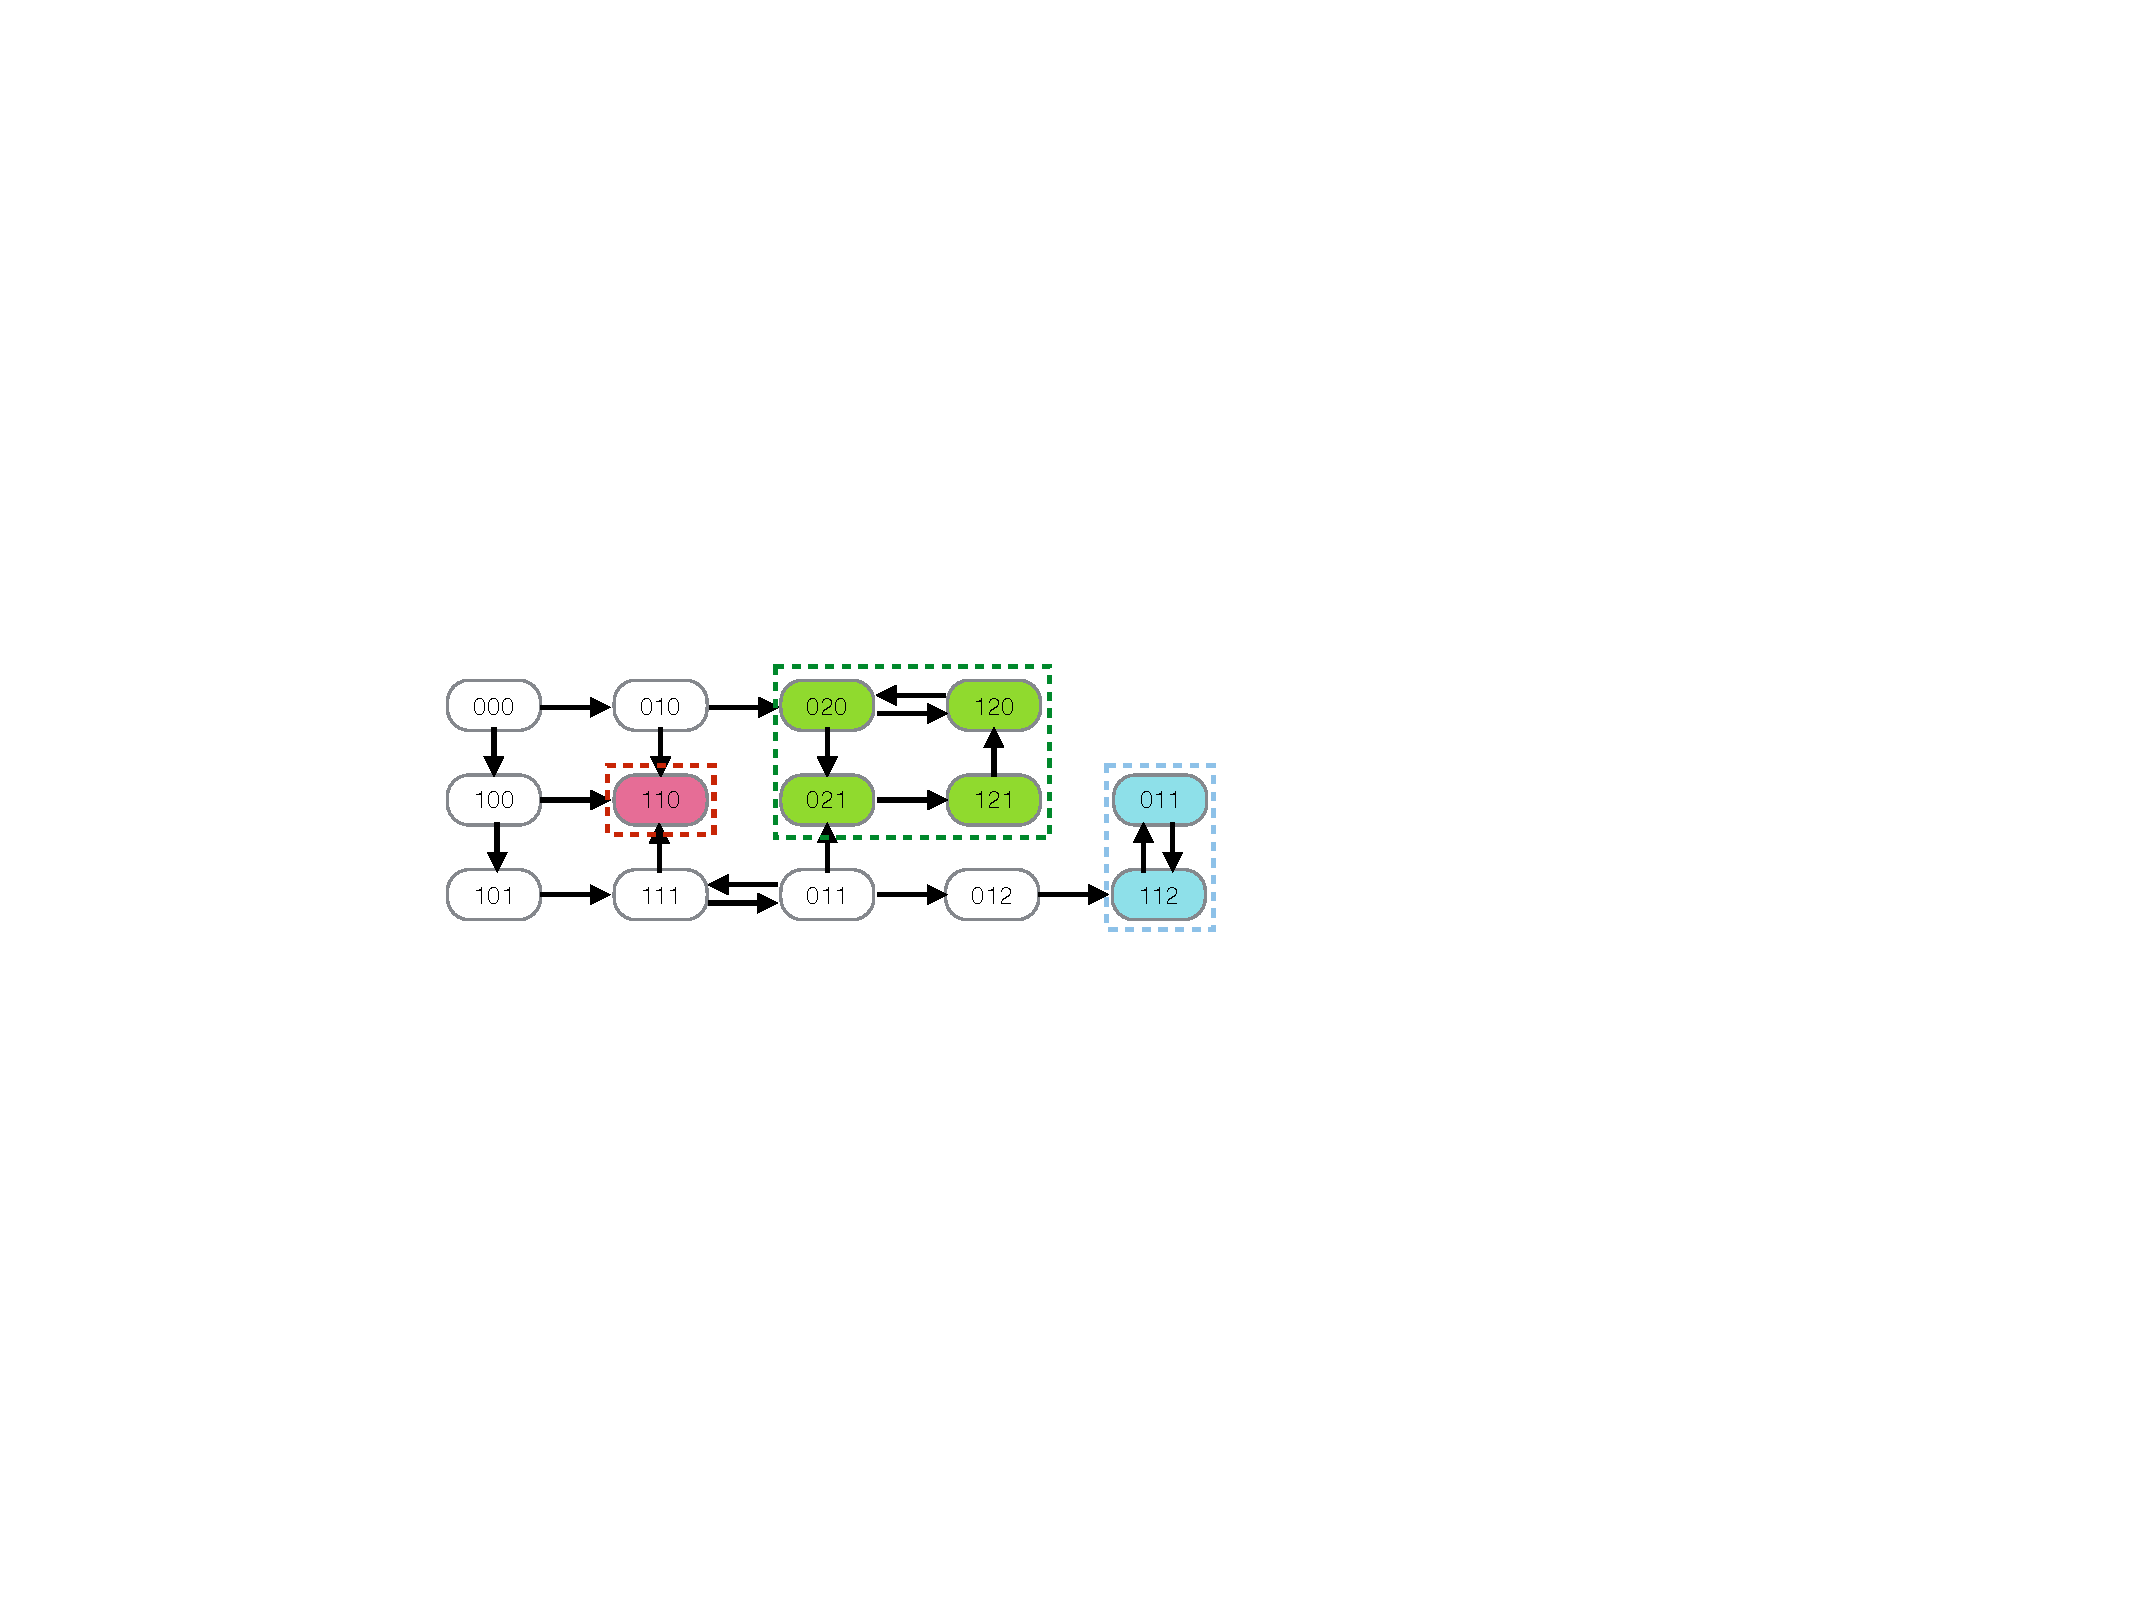
\includegraphics{figures/transition-graph.pdf}
\end{figure}


\section{Answer Set Programming}
\label{sec:asp}
\Emna{A revoir et parler d'avantage des contraintes}
In this section, we briefly recapitulate the basic elements of Answer Set Programming (ASP) \cite{baral2003knowledge}, a  declarative language that proved efficient to address highly computational problems. An answer set program is a finite set of rules of the form:
\begin{equation}
\label{asprule}
  a_{0}\ \leftarrow \ a_{1},\ \ldots,\ a_{m},\ not\ a_{m+1},\ \ldots,\ not\ a_{n}
\end{equation}
where $n \ge m \ge 0$, $a_{0}$ is a propositional atom or $\bot$, all
$a_{1}, \ldots ,a_{n}$ are propositional atoms, and the symbol ``$not$'' denotes  negation as failure.
The intuitive reading of such a rule is that whenever $a_{1}, \ldots, a_{m}$
are known to be true and there is no evidence for any of the negated atoms $a_{m+1}, \ldots, a_{n}$ to be true, then $a_{0}$ has to be true as well.
\label{constraint}
If $a_{0} = \bot$, then the rule becomes a constraint (in which case the symbol $\bot$ is usually omitted).
As $\bot$ can never become true, if the right-hand side of a constraint is validated, it invalidates the whole solution.

In the ASP paradigm, the search of solutions consists in computing the \emph{answer sets} of a given program.
An answer set for a program is defined by Gelfond and Lifschitz \cite{DBLP:conf/iclp/GelfondL88} as follows.
An \emph{interpretation} $I$ is a finite set of propositional atoms.
%An atom $a_i$ is \emph{true under $I$} if $a_i \in I$, and false otherwise.
A rule $r$ as given in \eqref{asprule} is \emph{true under~$I$} if and only if:
  \[\{a_1,\ \dots,\ a_{m}\} \subseteq I \wedge \{a_{m+1},\ \ldots,\ a_{n}\} \cap I = \emptyset \Rightarrow a_{0} \in I \enspace.\]
An interpretation $I$ is a \emph{model} of a program $P$ if each rule $r \in P$ is true under $I$.
Finally, $I$ is an answer set of $P$ if $I$ is a minimal (in terms of inclusion) model of $P^{I}$,
where $P^{I}$ is defined as the program that results from $P$ by deleting all rules that contain a negated atom that appears in $I$,
and deleting all negated atoms from the remaining rules.
Programs can yield no answer set, one answer set, or several answer sets.
To compute the answer sets of a given program, one needs a grounder (to remove variables from the rules) and a solver.
For the present work, we used \textsc{Clingo}\footnote{We used \textsc{Clingo} version 4.5.0: \url{http://potassco.sourceforge.net/}}~\cite{gebser2010incremental} which is a combination of both.

\medskip
In the rest of this paper, we use ASP to tackle the problems of enumerating all fixed points and attractors of a given PH model.


\section{Fixed point enumeration}
\label{sec:fixpoint}

The first aspect of our present work is the enumeration of a special kind of basins of attraction: fixed points (also called stable states or steady states) which are composed of only one state.
They can be studied separately from attractors because their enumeration follows a different pattern which is more specific to this problem.

\subsection{Translating a Process Hitting model into Answer Set Programming}
Before any analysis of the network,
we first need to translate it into ASP\benchmarksfootnote.
To do this, we use the self-describing predicates
\texttt{sort}, \texttt{process} and \texttt{action} to define the sorts, processes and actions of the network, respectively.
\pref{ex:asp-ph} shows how a PH network is defined with these predicates.

\begin{example}[Representation of a PH model in ASP]
\label{ex:asp-ph}
The representation of the PH model of \pref{fig:ph} in ASP is the following:
\begin{lstlisting}
process("a", 0..1). process("b", 0..2). process("c", 0..1). %\label{ASPprocess1}
process("d", 0..1).  process("e", 0..2). %\label{ASPprocess2}
sort(X) :- process(X,_). %\label{ASPsort}
action("d",1,"d",1,0). action("d",0,"a",0,1). %\label{actions1}
action("a",1,"c",1,"b",0,1). action("a",1,"b",1,"e",0,1). %\label{actions2}
\end{lstlisting}
In \refll{ASPprocess1}{ASPprocess2} we create the list of processes corresponding to each sort;
for example, the sort \texttt{"a"} has 2 processes numbered \texttt{0} and \texttt{1} and
predicate ``\texttt{process("a", 0..1).}'' will in fact expand into the two following predicates:
\addtocounter{lstnumber}{-1}
\begin{lstlisting}[numbers=none]
process("a", 0). process("a", 1).
\end{lstlisting}
\Refl{ASPsort} enumerates every sort of the network from the previous information.
In ASP, a word starting with a capital letter is a variable,
and the underscore (``\texttt{\_}'') is a placeholder for any value.
Finally, all the actions of the network are defined straightforwardly in \refll{actions1}{actions2};
for instance, the predicate ``\texttt{action("d",0,"a",0,1).}'' represents the action
$\PHfrappe{d_0}{a_0}{a_1}$ and we use the same predicate to define an action with several hitters, for instance: ``\texttt{action("a",1,"c",1,"b",0,1)}" to represent the action $\PHfrappe{a_1 \wedge c_1}{b_0}{b_1}$ meaning that when $a_1$ and $c_1$ are simultaneously active, they can cooperate to change the level of $b$ from $0$ to $1$.
\end{example}

\subsection{Search of fixed points}
% du blabla sur les points fxes

The enumeration of fixed points requires to translate the definition of a fixed point (given in \pref{def:fixpoint})
into logic rules for an ASP program. For this, the first step is to browse all possible states of the network,
that is, all possible combinations of processes by choosing exactly one process from each sort, which is done in \refl{selectprocesses}.
\begin{lstlisting}
1 {selectProc(A,I) : process(A,I)} 1 :- sort(A). %\label{selectprocesses}
\end{lstlisting}
This line constitutes a \emph{cardinality rule} which creates as many potential answer sets as the number of possible states
to take into account.
Cardinality rules are very useful to enumerate candidate answer sets,
and they allow to tune how many atom of each kind is included in every set.
In this particular case, we stated that a state (\texttt{selectProc})
is created by considering exactly one \texttt{process} for each existing \texttt{sort}.

The next step consists in filtering out any state, among all those generated,
that is not a fixed point.
In this case, it consists in eliminating all candidate answer sets
in which at least one action can be played.
For this, we use a constraint:
any solution that satisfies the body of this constraint will be removed from the answer set (because the atom $\bot$ cannot be true in an answer set, as explained in Page~\pageref{constraint}).
Regarding our problem, a state is eliminated if there exists a playable action in the considered state (\refll{constraintFix}{constraintFix2}). The first constraint (\refl{constraintFix}) treats the case of an action with only one hitter and the second (\refl{constraintFix2}) the actions with two hitters.
To generalize this, we developed a script that takes into account the maximum number of hitters of any action in the model and generates as many constraints as necessary.
\begin{lstlisting}
:- action(A,I,B,J,_), selectProc(A,I), selectProc(B,J), A!=B. %\label{constraintFix}
:- action(A1,I1,A2,I2,B,J,_), selectProc(A1,I1),selectProc(A2,I2), 
      selectProc(B,J), A!=B. %\label{constraintFix2}
\end{lstlisting}
Finally, the fixed points of the considered model are exactly the states represented in each remaining answer set,
described by the atoms \texttt{selectProc(A,I)}.

\begin{example}[Fixed points enumeration]
The PH model of \pref{fig:ph} contains 5 sorts:
$a$, $b$, $c$ and $d$ have 2 processes while $b$ has 3; therefore, the whole model has $2*2*2*3*3 = 72$ states (whether they can be reached or not from a given initial state).
We can check that this model contains exactly 5 fixed points: $\PHstate{a_1, b_0, c_0, d_0, e_1}$, $\PHstate{a_1, b_2, c_0, d_0, e_1}$, $\PHstate{a_1, b_1, c_0, d_0, e_1}$, $\PHstate{a_1, b_0, c_0, d_0, e_0}$, $\PHstate{a_1, b_2, c_0, d_0, e_0}$.
Indeed, there is no playable action in these states so no execution is possible from these. In this example, no other state verifies this property.

If we execute the ASP program detailed above (\refll{selectprocesses}{constraintFix2})
alongside with the description of the PH model given in \pref{ex:asp-ph} (\refll{ASPprocess1}{actions2}),
we obtain 5 answer sets that match the expected result.
The output of \textsc{Clingo} is the following:
%\begin{changemargin}{-2cm}{-1cm}
%\scriptsize{ 
\addtocounter{lstnumber}{-15}
\begin{lstlisting}[numbers=none]
Answer: 1
selectProc("a",1) selectProc("b",0) selectProc("c",0)
selectProc("d",0) selectProc("e",1)
Answer: 2
selectProc("a",1) selectProc("b",2) selectProc("c",0)
selectProc("d",0) selectProc("e",1)
Answer: 3
selectProc("a",1) selectProc("b",1) selectProc("c",0)
selectProc("d",0) selectProc("e",1)
Answer: 4
selectProc("a",1) selectProc("b",0) selectProc("c",0)
selectProc("d",0) selectProc("e",0)
Answer: 5
selectProc("a",1) selectProc("b",2) selectProc("c",0)
selectProc("d",0) selectProc("e",0)
\end{lstlisting}
%}
%\end{changemargin}
\end{example}

In \pref{alg:PH-fixpont} we give an imperative pseudocode
that corresponds to the computation of
all fixed points in a given PH network.
We give this algorithm only for educational purposes
as it may help a reader not accustomed with ASP to understand
what our implementation intends to do,
and the complexity of such an enumeration.
However, it is important to understand that
such an algorithm is never given to the solver,
which only considers ASP code as given in \refll{ASPprocess1}{constraintFix2}.

\begin{algorithm}[t]
  \caption{Enumeration of the fixed points of a PH}
  \label{alg:PH-fixpont}
  \begin{itemize}
    \item[] \textbf{INPUT:} A network $PH=(\PHs,\PHl,\PHa)$
    \item[] \textbf{OUTPUT:} All the fixed points (\ie steady states or attractors of size 1)
    \item[] \textbf{Initialization:} $\Delta \longleftarrow \varnothing$ \quad // Will be the set of fixed points
    \item[] \textbf{Begin:} \\
      \hspace{0.2cm}  \textbf{\textit{forall}} $\PHst_i \in \PHl$ \textbf{\textit{do}} 
        \begin{itemize}
          \item[] Compute the set $A_{\PHst_i}$ of all the playable actions in $\PHst_i$
          \item[] \textbf{\textit{if}} $A_{\PHst_i} = \varnothing$ \textbf{\textit{then}} \\
            \hspace{0.5cm}  $\Delta \longleftarrow \Delta \cup \{\PHst_i\}$ \\
           \textbf{\textit{end if}} 
        \end{itemize}   
      \hspace{0.2cm} \textbf{\textit{end forall}} \\    
      \hspace{0.2cm} \textbf{\textit{return}} $\Delta$    
  \end{itemize}
\end{algorithm}


\section{Fixed-size attractors enumeration}
\label{sec:attractors}
\subsection{Intuitive idea}
The computational method for finding attractors of size $N$ in an automata network falls into three stages:
\begin{enumerate}
  \item Enumerating all sub-State Transition Graphs (sub-STGs)
    with $N$ transitions,
  \item Filtering out all of these sub-STG that are not cyclic,
  \item Checking, for each state of the remaining cycles
    if all the next states are part of this cycle.
\end{enumerate}
Once all steps are passed, the only remaining sub-STGs are attractors of size $N$,
because they consist of cycles that cannot be escaped.

% Description de l'algo
\Maxime{Idem : expliquer les raisons de mettre l'algo.}
The pseudocode of the presented algorithm is given as Algorithm \ref{alg:PH-attractor}. We use ASP for the identification of all sub-STG with $N$ transitions in a multiple-valued network. \Maxime{C'est quoi un “multiple-valued network” ? “Multi-valued” ? Mais pourquoi le préciser ici, pourquoi ne pas juste dire “PH” ?} First, we generate a set of loops of size $N$. Then, a set satisfying the attractors formula corresponds to a valid solution. This process can be repeated iteratively for larger and larger values of $N$ until all attractors are identified.

%Faire un algo
\begin{algorithm}[!h]
	\caption{Enumarate Attractors of size $N$ from an Automata Network}
	\label{alg:PH-attractor}
	\begin{itemize}
		\item[] \textbf{INPUT}: Automata Network $PH=(\PHs,\PHl,\PHa)$, Attractor size $N$ // $N \geq 2$
		\item[] \textbf{OUTPUT}: All the attractors of size $N$
		\item[] \textbf{Initialize}: $\Delta_N \longleftarrow \varnothing$ // The set of the attractors of size $N$
		\item[] \textbf{Begin} \\
		
			\hspace{0.2cm}	\textbf{\textit{forall}} $\PHst_i \in \PHl$ \textbf{\textit{do}} 
				
				\begin{itemize}
					\item[] compute the $N$ successors: $\PHst_i \rightarrowtail ... \rightarrowtail \PHst_N$ \\ let $\Delta_N^i=$\{$\PHst_j \in \PHl, i \leq j \leq N$\} %be the set of these states
					
					\item[] \textbf{\textit{if}} $\PHst_0 = \PHst_N$ \textbf{\textit{then}} \\
						\hspace{0.7cm}  $loop(\Delta_N^i) \longleftarrow True$ \\
					 \textbf{\textit{else}} \\
					 	\hspace{0.7cm}  $loop(\Delta_N^i) \longleftarrow False$ \\
					 \textbf{\textit{end if}} 
					 
					\item[] \textbf{\textit{if}} $loop(\Delta_N^i) = True$ \textbf{\textit{then}} \\
					
%						\begin{itemize}
							\hspace{0.7cm} $attractor(\Delta_N^i) \longleftarrow True$	\\
							
							\hspace{0.7cm} \textbf{\textit{forall}} $\PHst_j \in \Delta_N^i$ \textbf{\textit{do}} \\
							
							\hspace{1.2cm} \textbf{\textit{if}} $\exists$ $\Sce(\PHst_j) \notin  \Delta_N^i$ \textbf{\textit{then}} \\ \hspace{1.7cm} $attractor(\Delta_N^i) \longleftarrow False$ \\
							\hspace{1.2cm} \textbf{\textit{end if}} 
							
							\textbf{\textit{else}} \\
							\hspace{0.7cm} $attractor(\Delta_N^i) \longleftarrow False$ \\
%						\end{itemize}		
							\textbf{\textit{end if}} 
														
					\item[] \textbf{\textit{if}} $attractor(\Delta_N^i) = True$ \textbf{\textit{then}}\\
						\hspace{0.7cm} \textbf{\textit{forall}} $\PHst_j, \PHst_k \in \Delta_N^i, j \neq k$ \textbf{\textit{do}} \\								
								\hspace{1.2cm} \textbf{\textit{if}} $loop(\Delta_k^j) = True$ \textbf{\textit{then}}\\
									\hspace{1.7cm} $complexLoop(\Delta_N^i) \longleftarrow False$ \\
									\hspace{1.7cm} $x \longleftarrow j+1$ \\									
									\hspace{1.7cm} \textbf{\textit{while}} $x \leq k-1 $ \textbf{\textit{and}} $complexLoop(\Delta_N^i) = False$ \textbf{\textit{do}} \\	
									
										\hspace{2.1cm} \textbf{\textit{if}} $loop(\Delta_{k+x}^{j+x}) = False$ \textbf{\textit{then}}\\
											\hspace{2.5cm} $complexLoop(\Delta_N^i) \longleftarrow True$ \\
										\hspace{2.1cm} \textbf{\textit{end if}} \\
									\hspace{1.7cm} \textbf{\textit{end while}} \\
								\hspace{1.2cm} \textbf{\textit{end if}} \\
						\hspace{0.7cm} \textbf{\textit{end forall}} 	\\

					\hspace{0.7cm} \textbf{\textit{if}} $complexLoop(\Delta_N^i) = False$ \textbf{\textit{then}}\\
						\hspace{1.2cm}  $attractor(\Delta_N^i) \longleftarrow False$\\
					\hspace{0.7cm} \textbf{\textit{end if}} 						
						
					\textbf{\textit{end if}} \\

					\item[] \textbf{\textit{if}} $attractor(\Delta_N^i) = True$ \textbf{\textit{then}}\\
					\hspace{0.5cm}  $\Delta_N \longleftarrow \Delta_N \cup \Delta_N^i$ \\
					\textbf{\textit{end if}} 

				\end{itemize}		
			\hspace{0.2cm} \textbf{\textit{end forall}} \\		
			\hspace{0.2cm} \textbf{\textit{return}} $\Delta_N$		
	\end{itemize}
\end{algorithm}

% Mettre du code ASP + explication
\subsection{Cycles enumeration}
The presented algorithm searches for all sub-graphs with a given number $N$ of transitions %(i.e path of length $N$)
in the network. As we start each time from a different initial state to simulate the evolution of the model, it means that in the end we browse all the model and generate all possible states (\refl{selectprocesses}). 

The evolution of a model is done in a limited number of steps $N$. At the beginning of an ASP program we can define constants whose values will be choosen by the user every time he execute it. Here we use \texttt{n} as a constant that defines the number of states we want to have.
We therefore define the predicate \texttt{state(0..n)}.
For example, \texttt{state(0..5)} will compute the 6 successive states, including the initial state.

The dynamics of a network is described by its actions; therefore, identifying the future states requires to first identify the playable actions for each state. We remind that an action is playable in a state when all its hitter processes and target process are active in this state (see Definition \ref{def:playableAction}). Therefore, we define an ASP predicate $\texttt{playable(action(A}_\texttt{1}\texttt{,I}_\texttt{1}\texttt{,...,A}_\texttt{n}\texttt{,I}_\texttt{n}\texttt{, B,J,K),S)}$ which is true when the processes  ${\texttt{A}_\texttt{1}}_{\texttt{I}_\texttt{1}}\texttt{,...,}{\texttt{A}_\texttt{n}}_{\texttt{I}_\texttt{n}}$ and $\texttt{B}_\texttt{J}$ are active at state \texttt{S}.

The cardinality rule of \refl{e2a}
creates a set of as many predicates as there are possible simulations from the chosen state,
thus reproducing all possible branchings in the possible simulations of the model, in the form of as many potential answer sets. It is also needed to enforce the strictly \emph{asynchronous} dynamic
which forces that exactly one process can change between two states and keeping the non-deterministic property.
To remove all scenarios where two or more actions have been played between
two states, we use the constraint of \refl{e2b}.
Thus, the remaining scenarios contained in the answer sets all strictly follow
the asynchronous dynamics of the Automata Networs.
We finally witness that the active expression level of sort \texttt{B} has changed between states \texttt{S} and \texttt{S+1} with the predicate \texttt{change(B,S+1)} of \refll{e3a}{e3b}. We create as much as necessary rules to find the changed sort that is the result of an action having one or more hitters (here we detailed action with 1 and 2 hitters).

\begin{lstlisting}
1{play(Action,S)}1 :- playable(Action,S), state(S). %\label{e2a} 
:- 2{play(Action,S)}, state(S). %\label{e2b}
change(B,S+1) :- play(action(_,_,B,_,_),T), state(S). %\label{e3a}
change(B,S+1) :- play(action(_,_,_,_,B,_,_),T), state(S). %\label{e3b}
\end{lstlisting}

Finally, the active processes at state \texttt{S+1},
thus representing the next state in the dynamics, depending on the chosen bounce,
can be computed by the rules of \refll{e4}{e5a}.
\begin{lstlisting}
instate(activeProc(B,K),S+1) :-  play(action(_,_,B,_,K),S), state(S).%\label{e4}
instate(activeProc(B,K),S+1) :-  instate(activeProc(B,K),S),%\label{e5}
				  not change(B,S+1), state(S).%\label{e5a}
\end{lstlisting}
In other words, the state of state \texttt{S+1} contains one updated active process $\texttt{B}_\texttt{K}$
resulting from the predicate \texttt{play(action(\_,\_,B,\_,K),T)} (\refl{e4})
as well as all the unchanged processes that correspond to the other sorts (\refll{e5}{e5a}).

The overall result of the pieces of program presented in this subsection
is an answer set containing one answer for each
possible simulation in \texttt{n} time steps,
starting from each state.
As a result, it reproduces all sub-STG of size $N$.
%%%%%%%%%%%

Once a sub-STG is found, we check whether it is a cycle (i.e a loop) or not. 
To do so, we use the predicate \texttt{getNbrRepetition(X,S1,S2)} which permits to get the number \texttt{X} of identical active processes between two tates \texttt{S1} et \texttt{S2}. This predicate refers to another predicate, \texttt{repeter(P,S1,S2)} (\refll{repeter1}{repeter2}), that is true for each process which is active at both \texttt{S1} and \texttt{S2}. 
\begin{lstlisting}
repeter(P,S1,S2) :- selectProcSt(P,S1), selectProcSt(P,S2), %\label{repeter1}
state(S1), state(S2). %\label{repeter2}
getNbrRepetition(X,S1,S2) :- X={repeter(F,S1,S2)}, S1!=S2, %\label{getRep1}
state(S1), state(S2). %\label{getRep2}
\end{lstlisting}
Then computing the number of repeated processes between \texttt{S1} and \texttt{S2} in \refll{getRep1}{getRep2} will permit to us to compare this number with the total number of sorts, which is the maximum number of repetition, and determine if there is a loop between the two states. In our case we just need to compare the first state (\texttt{S1=0}) and the last state (\texttt{S2=n}) of the sub-STG. Therefore we eliminate all sub-STG that are not cycles by the constraint (\refl{loop}).
\Maxime{Cette partie mériterait d'être un peu mieux expliquée.}
\begin{lstlisting}
:- loop(0, n)  %\label{loop}
\end{lstlisting}

\subsection{Attractors enumation}
\Maxime{Tout le début de cette section n'est pas très clair et mériterait aussi d'être clarifié et reformulé.}
Since each state of the STG of an automata network has various next states (due to the non-deterministic dynamics), a cyclic sub-STG is not necessarily an attractor. Thus, we first need to determine the presence of a cycle by checking whether the first state and the last state of the sub-STG are the same. Then we check if this sub-STG is an attractor. 
Filtering the remaining sub-STGs means using a constraint in ASP. Indeed a constraint has many advanges for such NP-Hard problems. Indeed, it permits to decrease the computational time. But to benifit of this specific type of logic rules, we have to think oppositly and present the opposite of what we are looking for. 
In our case, to say that a cycle is not an attractor, it means that it has at least one state that has a successor which is not apart of it (\refl{existOut}).
\begin{lstlisting}
:- existActionOut.  %\label{existOut}
\end{lstlisting}
It is necessary now to compute all playble actions for each state $\texttt{S}_\texttt{i}$ between the states \texttt{0} and \texttt{n}. For that we propose a similar rule to \refl{e2a} but with different predicate name and different parameters: \texttt{candidatePlayable(Action,S)}. It is true when an action \texttt{Action} is playable at state \texttt{S} which is between \texttt{0} and \texttt{n}. Also this action should be different from the action that was played in the cycle transforming the system from \texttt{S} to \texttt{S+1} that is also a part of the cycle (\refll{comptPlayAct}{candidatPlayAct}).
\begin{lstlisting}
firstCandidatePlayable(action(A,I,B,J,K),S) :- action(A,I,B,J,K), %\label{comptPlayAct}
		selectProcSt(activeProc(B,J),S), selectProcSt(activeProc(A,I),S), 
		loop(0, n), S>0, S<n, state(S).		
candidatePlayable(Action1,S) :- firstCandidatePlayable(Action1,S), 
		playable(Action2,S), Action1!= Action2.	%\label{candidatPlayAct}
\end{lstlisting}
After finding the candidate playable actions in each state of the cycle, it remains to verify if the result states are already a part of the cycle or if there are new states. Indeed it is possible to have other playable actions in the cycle (\texttt{playableInCycle}, \refll{playIncyc1}{playIncyc3}) but these actions lead to the same states. It confirms that the model indefinitely cycles in these states. Once all playable actions are checked whatever they leads to a state in the cycle or not, the predicate \texttt{existActionOut} is verified when at least one action could envolve the system to a state out of the cycle (\refl{existActOut1}).
\begin{lstlisting}
playableInCycle(action(A,I,B,J,K),S) :- candidatePlayable(action(A,I,B,J,K),S), %\label{playIncyc1}
	selectProcSt(activeProc(B,K),Si), Si>=0, Si<=n, Si!=S+1, %\label{playIncyc2}
	getNbrRepetition(X,S,Si), getNbreSorts(Y), Y==X+1, state(Si). %\label{playIncyc3}
existActionOut :- candidatePlayable(Action,S), not playableInCycle(Action,S). %\label{existActOut1}
\end{lstlisting}

At this step, we want to ensure that the considered attractor is of size $N$, and not of a size which is a divisor of $N$. The idea, as described in Algorithm \ref{alg:PH-attractor} and \refll{loopX}{constraintloopX}, is to filter the repeated loops out of the result. For this, we define the predicate \texttt{loopX(S1,S2,X)} which becomes true if there is a loop between the \texttt{X}\textsuperscript{th} successor of \texttt{S1} and the \texttt{X}\textsuperscript{th} successor of \texttt{S2} in the considered succession of states. This predicate is a clue that the same loop may have been traversed twice. In \texttt{notloopX(S1,S2)} we state that there exists at least one \texttt{X}\textsuperscript{th} successor of \texttt{S1} that does not loop back to the \texttt{X}\textsuperscript{th} successor of \texttt{S2}. Finally with the constraint in \refl{constraintloopX}, we eliminate the case of having the repeated loops.

\begin{lstlisting}
loopX(S1,S2,X) :- loop(S1+X, S2+X), 0<=X, X<=S2-S1, state(S1;S2;X). %\label{loopX}
notloopX(S1,S2) :- not loopX(S1,S2,X), 0<=X, X<=S2-S1, state(S1;S2;X). %\label{notloopX}
:- loop(S1,S2), loop(S1, S2+(S2-S1)), not notloopX(S1,S2). %\label{constraintloopX}
\end{lstlisting}

The problem of finding attractors in a multi-valued automata network is NP-hard. However, we have good results when the algorithm \ref{alg:PH-attractor} is developed with ASP \Maxime{Je ne suis pas d'accord : on ne traduit pas cet algorithme en ASP ! On écrit autre chose qui doit nous donner un résultat équivalent, mais ce n'est pas un algorithme impératif}. Indeed, we show in Section \ref{sec:results}, by performing a number of computational experiments on biological networks, that the program can tackle even large systems and return a result in few seconds.

%
%
%Clearly, all states between any two occurrences of the last state belong to a loop. A loop corresponds to an attractor. We mark all attractor’s states. In the following iterations, we will only search for paths in which the last state is not marked.
%Until at least one attractor remains unmarked, we can find a path of any length since we can cycle in an attractor forever. However, once all attractors are identified and marked, we will only be able find paths which are shorter than a given length (at most the diameter of the STG). So, when we search for a path of some length k and it does not exist, this means that all attractors are already identified and the algorithm can terminate.
%If a path of length k does exist and it is loop-free, we double k and continue the search for a path of the new length.
%We illustrate the algorithm on the example of the Boolean network in Figure 1. The algorithm starts from searching for a path of length $N = 3$


% Pas sure de laisser cette partie on peut la mettre dans un autre article + une étude approffondie (bifurcation ou autre...)
%\section{Reachability of attractors }
%\label{sec:reach-attractor}
%\input{parts/reach-attractors}

\section{Results }
\label{sec:results}
% Section des résultat: Application sur des réseaux biologiques

The time complexities estimated from the results of computational experiments are a little different from those obtained by theoretical analysis. \Maxime{Qu'est-ce que la phrase précédente signifie ? Qu'entend-on par “theoretical analysis” ?} However, this is reasonable since, in our theoretical analysis, we assumed that the number of genes is very large.
%In this section, we. 
All experiments were run on a PC with Pentium VII 3 GHz processor and 16 Go memory.

\subsection{Lambda Phage model}
\begin{figure}[h]
   \caption{\label{fig:lambda-graph} 
   The figures are taken from \cite{thieffry1995dynamical,chaouiya2008petri} of the Lambda phage model. The left one presents the regulatory graph with positive and negative regulations represented by ’$+$’ and ’$-$’ signs. The second is the corresponding state transition graph (STG).% colored according to strongly connected components. 
We have two attractors: $(2000)$ is an attractor of size $1$ i.e a fixed point and $\{(0300), (0200)\}$ is an attractor of size $2$.}
   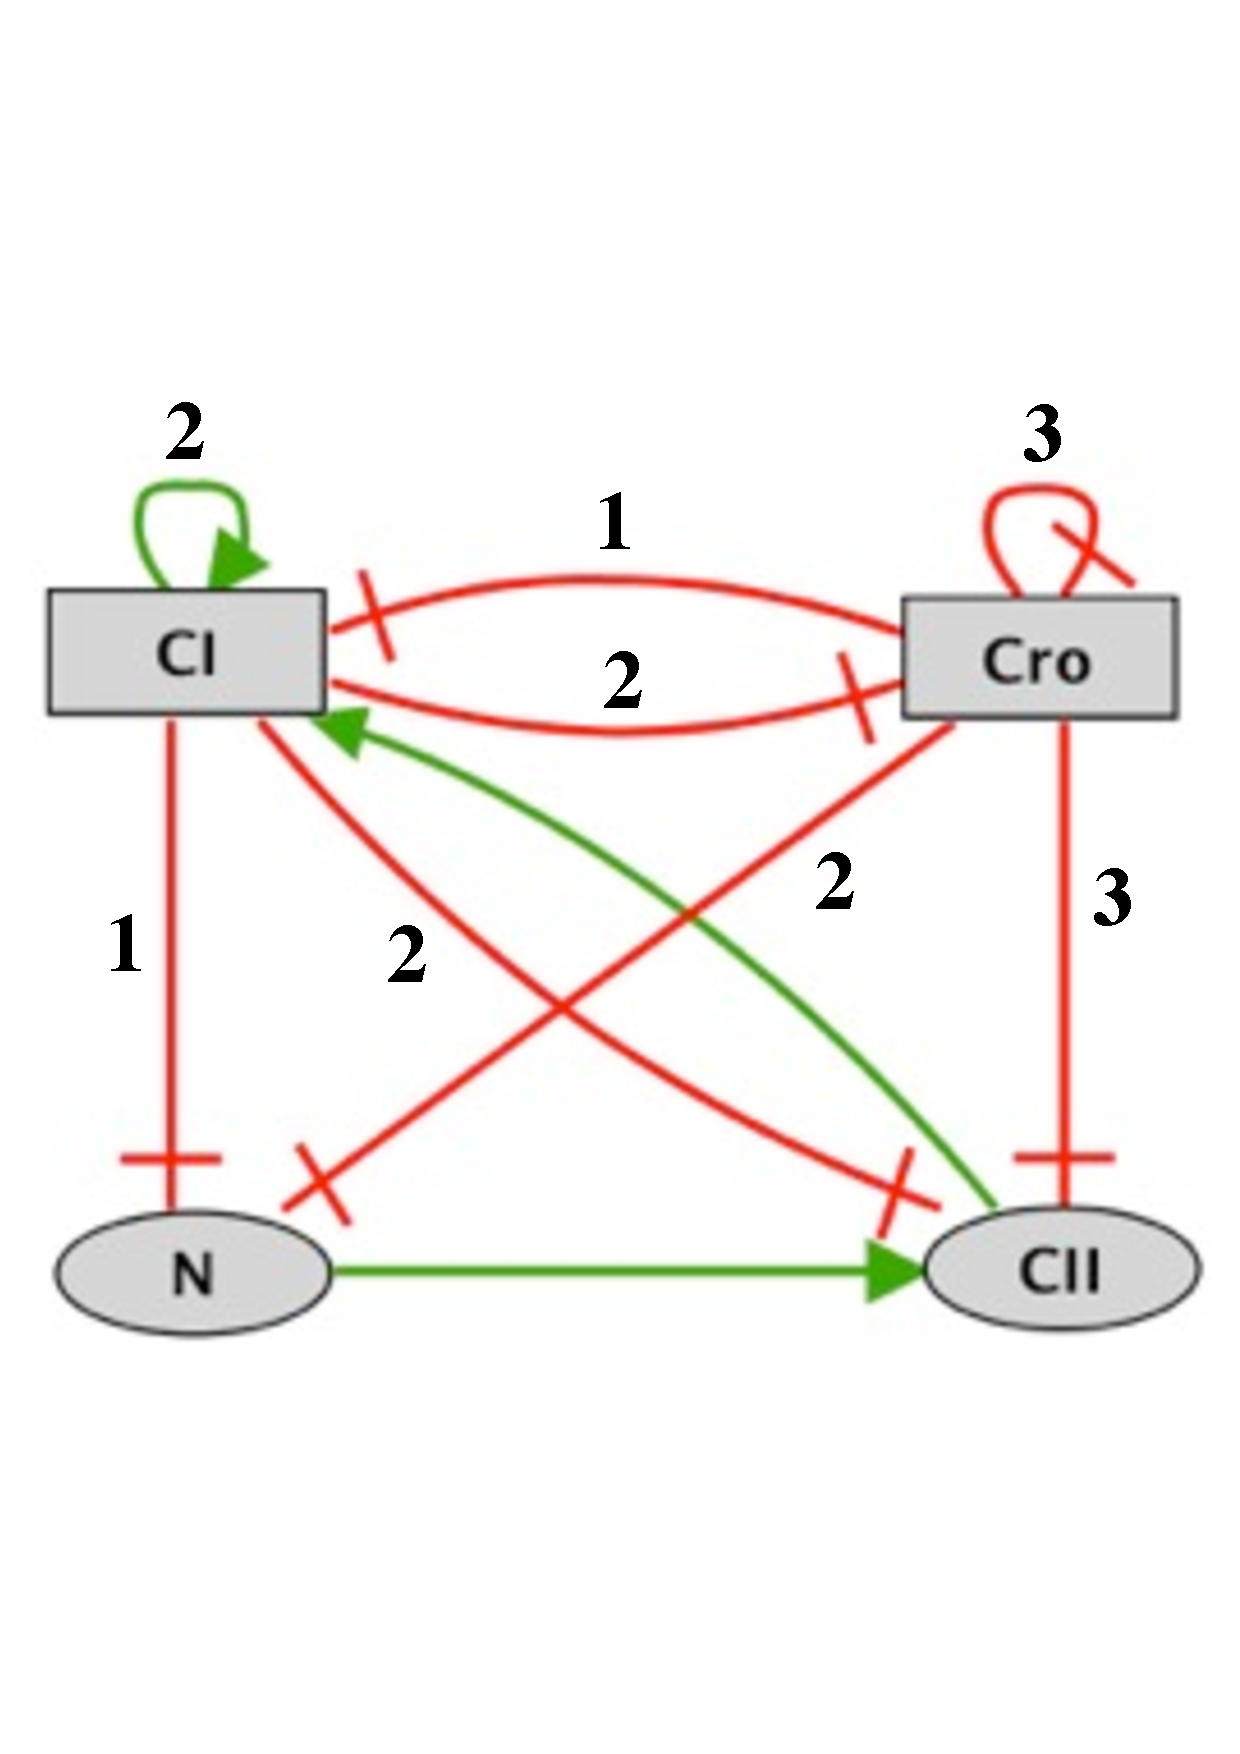
\includegraphics{figures/lampdaphage-thomas.pdf}
   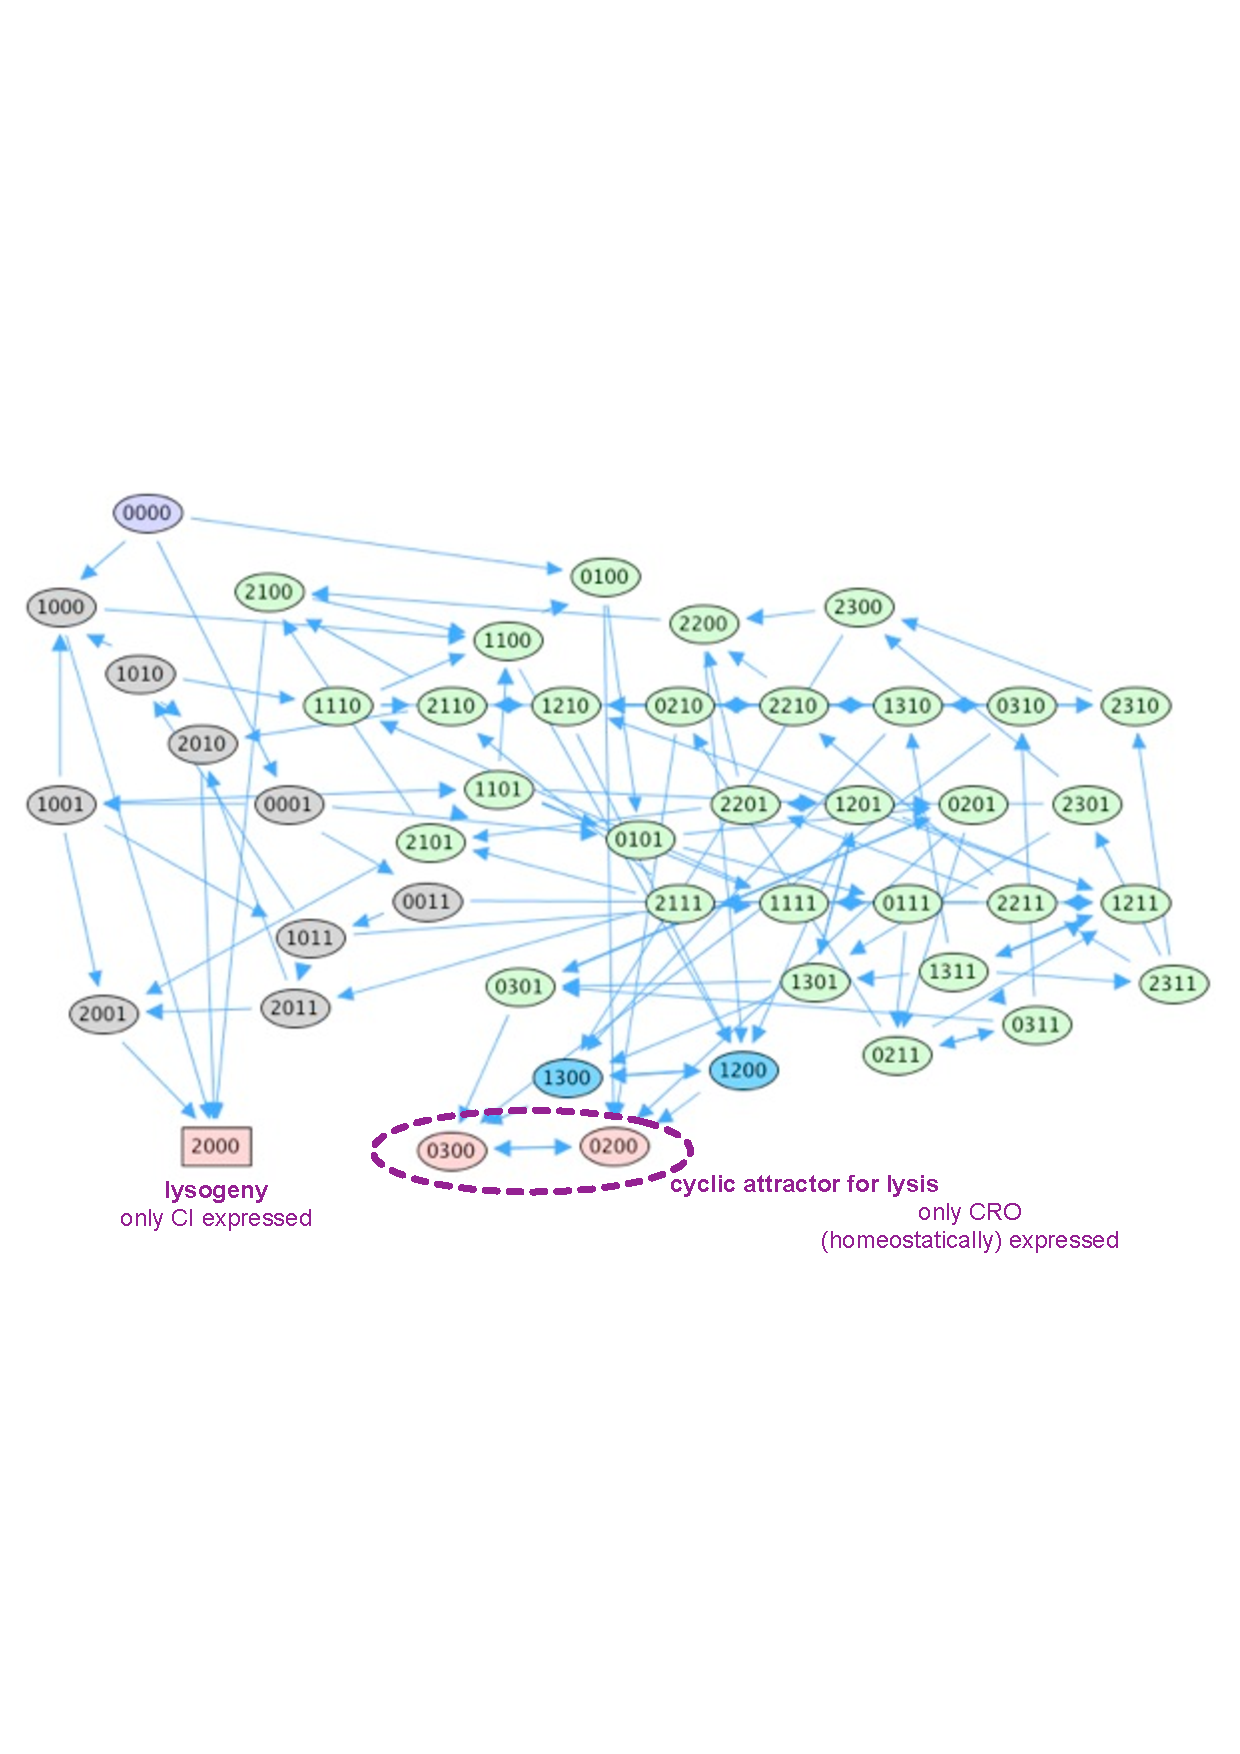
\includegraphics{figures/lampdaphage-STG.pdf}
\end{figure}

Like mentioned above, using our method we are not obliged to have the whole State Transition Graph. So that for finding these attractors (size $1$ and size $2$), it sufficient to compute only graphs of size $2$.
\Maxime{Ici, il faudrait répéter certains éléments de la description de la Figure 3 pour une meilleure compréhension.}

This network was modeled into an Automata Network ($4$ sorts, $48$ processes and $49$ actions) to be analysed later. The result that we get are the following: \\
\textit{ Lambda Phage Fixed points:} $\PHstate{CI_2, CII_0, Cro_0, N_0}$
\begin{lstlisting}[numbers=none]
Answer: 1
selectProc("CI",2) selectProc("CII",0) selectProc("Cro",0) selectProc("N",0)
\end{lstlisting}
\textit{Lambda Phage attractors of size $2$:} \{$\PHstate{CI_0, CII_0, Cro_2, N_0}$, $\PHstate{CI_0, CII_0, Cro_3, N_0}$ \}
\begin{lstlisting}[numbers=none]
Answer: 1
selectProcSt(activeProc("CI",0),0) selectProcSt(activeProc("CII",0),0)
selectProcSt(activeProc("Cro",2),0) selectProcSt(activeProc("N",0),0) 
selectProcSt(activeProc("CI",0),1) selectProcSt(activeProc("CII",0),1)
selectProcSt(activeProc("Cro",3),1) selectProcSt(activeProc("N",0),1)
 \end{lstlisting}

Thus we obtain $1$ answer set for each size that match the expected results. The program needed only $10$ms for finding the fixed point and $19$ms for the attractor.

\subsection{Benchmarks}
As benchmarks we use existing Multi-valued networks models of real organisms shown in Table \ref{tab:models}\benchmarksfootnote: the bacteriophage lambda phage \cite{thieffry1995dynamical}, the Hedgehog Signalling Pathway (\Emna{à revoir la réf} \cite{stecca2010context}), mTOR pathway in survival mechanisms \cite{javle2010inhibition} (\Emna{en cours de traduction}) and egf-tnf which is a mammalian signalling pathways induced by the Epidermal Growth Factor (EGF) and Tumour Necrosis Factor alpha (TNF$\alpha$) \cite{chaouiya2013sbml}.
We have constructed the input descriptions of these models, the automata networks, manually from the data in the corresponding papers.

\begin{changemargin}{-3cm}{-3cm}
\begin{center}
\begin{table*}[ht]
\begin{center}
\noindent%
%\begin{tabular}{| l| c | c | c ||>{\columncolor{verylightgray}} c | c ||>{\columncolor{verylightgray}}c | c | c ||}
\begin{tabular}{| l || c | c | c || c | c || c | c | c |}
\hline
\multicolumn{1}{| l ||}{Models} & \multicolumn{3}{c||}{PH representation} & \multicolumn{2}{c||}{Fixed points} & \multicolumn{3}{c|}{Attractors}\\
\hline
    & sorts & processes & states & sec &  \#results & sec & size & \#results \\
\hline
\hline
%  TTR  & 12 & 42  & $2^{19}$ & 0.004 & 0 & 0.004 & k & 0\\
%\hline
%  ERBB & 42 & 152 & $2^{70}$ & 0.017 & 3 & 0.004 & k & 0\\
%\hline
%  TCR & 54 & 156 & $2^{73}$ & 0.021 & 1 & 0.004 & k & 0\\
%\hline  
   \multirow{3}{*}{lambdaPhage}  & \multirow{3}{*}{4} & \multirow{3}{*}{11} & \multirow{3}{*}{48} & \multirow{3}{*}{0.003} & \multirow{3}{*}{1} & 0.019 & 2 & 1\\
 & & & & & & 0.033 & 4 & 0\\
 & & & & & & 0.470 & 20 & 0\\

\hline
 \multirow{3}{*}{hedgehog}  & \multirow{3}{*}{5} & \multirow{3}{*}{11} & \multirow{3}{*}{48} & \multirow{3}{*}{0.003} & \multirow{3}{*}{2} & 0.017 & 2 & 0\\
 & & & & & & 0.050 & 6 & 0\\
 & & & & & & 0.319 & 20 & 0\\
\hline
 \multirow{3}{*}{mTOR}  & \multirow{3}{*}{6} & \multirow{3}{*}{12} & \multirow{3}{*}{$2^6$} & \multirow{3}{*}{0.009} & \multirow{3}{*}{1} & 0.019 & 2 & 0\\
 & & & & & & 0.101 & 8 & 0\\
 & & & & & & 0.397s & 16 & 0\\

\hline
 \multirow{3}{*}{egf-tnf}  & \multirow{3}{*}{28} & \multirow{3}{*}{56} & \multirow{3}{*}{$2^{28}$} & \multirow{3}{*}{0.005} & \multirow{3}{*}{2} & 0 & 2 & 0\\
 & & & & & & 9.192 & 8 & 1\\
% & & & & & & xxx & xx & x\\
\hline
\end{tabular}
\vspace*{4pt}
\caption{\label{tab:models}%
Description of the models used in our tests and results of fixed points and attractors enumeration.
Each model is referred to by its short name, where
lambdaPhage stands for the bacteriophage lambda phage \cite{thieffry1995dynamical}, hedgehog for the Hedgehog Signalling Pathway \cite{stecca2010context}, mTOR for the pathway in survival mechanisms \cite{javle2010inhibition} and egf-tnf for the mammalian signalling pathways induced by the Epidermal Growth Factor (EGF) and Tumour Necrosis Factor alpha (TNF$\alpha$) \cite{chaouiya2013sbml}.
For each of them, this table gives the number of biological components
in the original representation,
and the number of sorts, the number of processes
and the number of states in the PH model.
Then, the next two columns give the computation time for the enumeration of all fixed points and the number of results returned. Finally, the last three columns give the computation time for the enumeration of all attractors, their size and the number of found attractors for each size.
}
\end{center}
\end{table*}
\end{center}
\end{changemargin}


\section{Conclusion and future directions}
\label{sec:ccl}
\Maxime{Début à revoir.}
This paper presents a new logical approach to compute attractors
in a particular class of automata networks.
This class encompasses qualitative asynchronous biological networks,
making all results especially applicable to the widespread Thomas modeling.

The point of the method developed in this article is the computation and
the enumeration of the attractors of such a network.
We present a particular method for attractors of size 1 (also called fixed points or steady states)
and a more general one for all attractors of given size $N \geq 2$.
The originality of our work consists in using ASP, a powerful declarative programming paradigm.
Thanks to the encoding we introduced, and the powerful heuristics developed in modern solvers, we are able to tackle the enumeration of fixed points, cycles and attractors of medium-sized models.
The major benefit of such a method is to get an exhaustive enumeration of all potential states while still being tractable for models with dozens of interacting components.
Identifying attractors in large biological networks is a big challenge because it gives an insight to the long-term behavior of biological systems,
and we hope our work helps open new ways and tools to explore this field.

\Maxime{Il faudrait peut-être étoffer un peu la conclusion.}

\Maxime{Et ajouter des perspectives.}

%Perspective: The attractor inverse problem, which involves construct- ing BNs possessing a given attractor structure, is important to network inference from steady-state data. Most microarray- based gene-expression studies do not involve controlled tem- poral experimental data; rather, it is assumed that the data result from sampling from the steady state. Under the BN model, this means that the data come from the attractors.

%In this paper, we proposed a new logical approach to address some dynamical properties of Process Hitting models.
%The originality of our work consists in using ASP, a powerful declarative programming paradigm.
%Thanks to the encoding we introduced, we are not only able to tackle the enumeration of fixed points but also to check reachability properties.
%The major benefit of such a method is to get an exhaustive enumeration of all corresponding paths while still being tractable for models with dozens of interacting components.
%
%One of the perspectives of our work is to extend the set of models on which our approach could be applied. We can consider the addition of priorities or neutralizing edges, or tackle other representations,
%such as Thomas modeling~\cite{Thomas73}.
%However, the range of the analysis can also be enriched,
%by searching the set of initial states
%allowing to reach a given goal instead of the other way around,
%or extending the method to universal properties (like the $\mathsf{AF}$ operator in CTL).



%%%%%%%%%%%%%%%%%%%%%%%%%%%%%%%%%%%%%%%%%%%%%%%%%%%%%%%%%%%%%
%%                  The Bibliography                       %%
%%                                                         %%
%%  Bmc_mathpys.bst  will be used to                       %%
%%  create a .BBL file for submission.                     %%
%%  After submission of the .TEX file,                     %%
%%  you will be prompted to submit your .BBL file.         %%
%%                                                         %%
%%                                                         %%
%%  Note that the displayed Bibliography will not          %%
%%  necessarily be rendered by Latex exactly as specified  %%
%%  in the online Instructions for Authors.                %%
%%                                                         %%
%%%%%%%%%%%%%%%%%%%%%%%%%%%%%%%%%%%%%%%%%%%%%%%%%%%%%%%%%%%%%

% if your bibliography is in bibtex format, use those commands:
\bibliographystyle{bmc-mathphys} % Style BST file (bmc-mathphys, vancouver, spbasic).
\bibliography{biblio}      % Bibliography file (usually '*.bib' )
% for author-year bibliography (bmc-mathphys or spbasic)
% a) write to bib file (bmc-mathphys only)
% @settings{label, options="nameyear"}
% b) uncomment next line
%\nocite{label}


\end{document}
